%%
% Copyright (c) 2017 - 2024, Pascal Wagler;
% Copyright (c) 2014 - 2024, John MacFarlane
%
% All rights reserved.
%
% Redistribution and use in source and binary forms, with or without
% modification, are permitted provided that the following conditions
% are met:
%
% - Redistributions of source code must retain the above copyright
% notice, this list of conditions and the following disclaimer.
%
% - Redistributions in binary form must reproduce the above copyright
% notice, this list of conditions and the following disclaimer in the
% documentation and/or other materials provided with the distribution.
%
% - Neither the name of John MacFarlane nor the names of other
% contributors may be used to endorse or promote products derived
% from this software without specific prior written permission.
%
% THIS SOFTWARE IS PROVIDED BY THE COPYRIGHT HOLDERS AND CONTRIBUTORS
% "AS IS" AND ANY EXPRESS OR IMPLIED WARRANTIES, INCLUDING, BUT NOT
% LIMITED TO, THE IMPLIED WARRANTIES OF MERCHANTABILITY AND FITNESS
% FOR A PARTICULAR PURPOSE ARE DISCLAIMED. IN NO EVENT SHALL THE
% COPYRIGHT OWNER OR CONTRIBUTORS BE LIABLE FOR ANY DIRECT, INDIRECT,
% INCIDENTAL, SPECIAL, EXEMPLARY, OR CONSEQUENTIAL DAMAGES (INCLUDING,
% BUT NOT LIMITED TO, PROCUREMENT OF SUBSTITUTE GOODS OR SERVICES;
% LOSS OF USE, DATA, OR PROFITS; OR BUSINESS INTERRUPTION) HOWEVER
% CAUSED AND ON ANY THEORY OF LIABILITY, WHETHER IN CONTRACT, STRICT
% LIABILITY, OR TORT (INCLUDING NEGLIGENCE OR OTHERWISE) ARISING IN
% ANY WAY OUT OF THE USE OF THIS SOFTWARE, EVEN IF ADVISED OF THE
% POSSIBILITY OF SUCH DAMAGE.
%%

%%
% This is the Eisvogel pandoc LaTeX template.
%
% For usage information and examples visit the official GitHub page:
% https://github.com/Wandmalfarbe/pandoc-latex-template
%%

% Options for packages loaded elsewhere
\PassOptionsToPackage{unicode}{hyperref}
\PassOptionsToPackage{hyphens}{url}
\PassOptionsToPackage{dvipsnames,svgnames,x11names,table}{xcolor}
%
\documentclass[
  paper=a4,
  ,captions=tableheading
]{scrartcl}
\usepackage{amsmath,amssymb}
% Use setspace anyway because we change the default line spacing.
% The spacing is changed early to affect the titlepage and the TOC.
\usepackage{setspace}
\setstretch{1.2}
\usepackage{iftex}
\ifPDFTeX
  \usepackage[T1]{fontenc}
  \usepackage[utf8]{inputenc}
  \usepackage{textcomp} % provide euro and other symbols
\else % if luatex or xetex
  \usepackage{unicode-math} % this also loads fontspec
  \defaultfontfeatures{Scale=MatchLowercase}
  \defaultfontfeatures[\rmfamily]{Ligatures=TeX,Scale=1}
\fi
\usepackage{lmodern}
\ifPDFTeX\else
  % xetex/luatex font selection
\fi
% Use upquote if available, for straight quotes in verbatim environments
\IfFileExists{upquote.sty}{\usepackage{upquote}}{}
\IfFileExists{microtype.sty}{% use microtype if available
  \usepackage[]{microtype}
  \UseMicrotypeSet[protrusion]{basicmath} % disable protrusion for tt fonts
}{}
\makeatletter
\@ifundefined{KOMAClassName}{% if non-KOMA class
  \IfFileExists{parskip.sty}{%
    \usepackage{parskip}
  }{% else
    \setlength{\parindent}{0pt}
    \setlength{\parskip}{6pt plus 2pt minus 1pt}}
}{% if KOMA class
  \KOMAoptions{parskip=half}}
\makeatother
\usepackage{xcolor}
\definecolor{default-linkcolor}{HTML}{A50000}
\definecolor{default-filecolor}{HTML}{A50000}
\definecolor{default-citecolor}{HTML}{4077C0}
\definecolor{default-urlcolor}{HTML}{4077C0}
\usepackage[top=1in,bottom=1in]{geometry}
\usepackage{longtable,booktabs,array}
\usepackage{calc} % for calculating minipage widths
% Correct order of tables after \paragraph or \subparagraph
\usepackage{etoolbox}
\makeatletter
\patchcmd\longtable{\par}{\if@noskipsec\mbox{}\fi\par}{}{}
\makeatother
% Allow footnotes in longtable head/foot
\IfFileExists{footnotehyper.sty}{\usepackage{footnotehyper}}{\usepackage{footnote}}
\makesavenoteenv{longtable}
% add backlinks to footnote references, cf. https://tex.stackexchange.com/questions/302266/make-footnote-clickable-both-ways
\usepackage{footnotebackref}
\usepackage{graphicx}
\makeatletter
\newsavebox\pandoc@box
\newcommand*\pandocbounded[1]{% scales image to fit in text height/width
  \sbox\pandoc@box{#1}%
  \Gscale@div\@tempa{\textheight}{\dimexpr\ht\pandoc@box+\dp\pandoc@box\relax}%
  \Gscale@div\@tempb{\linewidth}{\wd\pandoc@box}%
  \ifdim\@tempb\p@<\@tempa\p@\let\@tempa\@tempb\fi% select the smaller of both
  \ifdim\@tempa\p@<\p@\scalebox{\@tempa}{\usebox\pandoc@box}%
  \else\usebox{\pandoc@box}%
  \fi%
}
% Set default figure placement to htbp
% Make use of float-package and set default placement for figures to H.
% The option H means 'PUT IT HERE' (as  opposed to the standard h option which means 'You may put it here if you like').
\usepackage{float}
\floatplacement{figure}{H}
\makeatother
\setlength{\emergencystretch}{3em} % prevent overfull lines
\providecommand{\tightlist}{%
  \setlength{\itemsep}{0pt}\setlength{\parskip}{0pt}}
\setcounter{secnumdepth}{-\maxdimen} % remove section numbering
\ifLuaTeX
\usepackage[bidi=basic]{babel}
\else
\usepackage[bidi=default]{babel}
\fi
\babelprovide[main,import]{english}
% get rid of language-specific shorthands (see #6817):
\let\LanguageShortHands\languageshorthands
\def\languageshorthands#1{}
\makeatletter
\@ifpackageloaded{subfig}{}{\usepackage{subfig}}
\@ifpackageloaded{caption}{}{\usepackage{caption}}
\captionsetup[subfloat]{margin=0.5em}
\AtBeginDocument{%
\renewcommand*\figurename{Figura}
\renewcommand*\tablename{Tabla}
}
\AtBeginDocument{%
\renewcommand*\listfigurename{Lista de Figuras}
\renewcommand*\listtablename{Lista de Tablas}
}
\newcounter{pandoccrossref@subfigures@footnote@counter}
\newenvironment{pandoccrossrefsubfigures}{%
\setcounter{pandoccrossref@subfigures@footnote@counter}{0}
\begin{figure}\centering%
\gdef\global@pandoccrossref@subfigures@footnotes{}%
\DeclareRobustCommand{\footnote}[1]{\footnotemark%
\stepcounter{pandoccrossref@subfigures@footnote@counter}%
\ifx\global@pandoccrossref@subfigures@footnotes\empty%
\gdef\global@pandoccrossref@subfigures@footnotes{{##1}}%
\else%
\g@addto@macro\global@pandoccrossref@subfigures@footnotes{, {##1}}%
\fi}}%
{\end{figure}%
\addtocounter{footnote}{-\value{pandoccrossref@subfigures@footnote@counter}}
\@for\f:=\global@pandoccrossref@subfigures@footnotes\do{\stepcounter{footnote}\footnotetext{\f}}%
\gdef\global@pandoccrossref@subfigures@footnotes{}}
\@ifpackageloaded{float}{}{\usepackage{float}}
\floatstyle{ruled}
\@ifundefined{c@chapter}{\newfloat{codelisting}{h}{lop}}{\newfloat{codelisting}{h}{lop}[chapter]}
\floatname{codelisting}{Listing}
\newcommand*\listoflistings{\listof{codelisting}{Listas del Documento}}
\makeatother
\usepackage{bookmark}
\IfFileExists{xurl.sty}{\usepackage{xurl}}{} % add URL line breaks if available
\urlstyle{same}
\hypersetup{
  pdftitle={Proyecto de Interoperabilidad JEP, 2024},
  pdflang={en},
  pdfsubject={Implementación Proyecto},
  pdfkeywords={Integración, Interoperabilidad, JEP, Softgic},
  hidelinks,
  breaklinks=true,
  pdfcreator={LaTeX via pandoc with the Eisvogel template}}
\title{Proyecto de Interoperabilidad JEP, 2024}
\usepackage{etoolbox}
\makeatletter
\providecommand{\subtitle}[1]{% add subtitle to \maketitle
  \apptocmd{\@title}{\par {\large #1 \par}}{}{}
}
\makeatother
\subtitle{Implementación Proyecto Evolución de Interoperabilidad JEP,
Softgic}
\author{}
\date{2024-09-16}



%%
%% added
%%


%
% for the background color of the title page
%
\usepackage{pagecolor}
\usepackage{afterpage}

%
% break urls
%
\PassOptionsToPackage{hyphens}{url}

%
% When using babel or polyglossia with biblatex, loading csquotes is recommended
% to ensure that quoted texts are typeset according to the rules of your main language.
%
\usepackage{csquotes}

%
% captions
%
\definecolor{caption-color}{HTML}{777777}
\usepackage[font={stretch=1.2}, textfont={color=caption-color}, position=top, skip=4mm, labelfont=bf, singlelinecheck=false, justification=raggedright]{caption}
\setcapindent{0em}

%
% blockquote
%
\definecolor{blockquote-border}{RGB}{221,221,221}
\definecolor{blockquote-text}{RGB}{119,119,119}
\usepackage{mdframed}
\newmdenv[rightline=false,bottomline=false,topline=false,linewidth=3pt,linecolor=blockquote-border,skipabove=\parskip]{customblockquote}
\renewenvironment{quote}{\begin{customblockquote}\list{}{\rightmargin=0em\leftmargin=0em}%
\item\relax\color{blockquote-text}\ignorespaces}{\unskip\unskip\endlist\end{customblockquote}}

%
% Source Sans Pro as the default font family
% Source Code Pro for monospace text
%
% 'default' option sets the default
% font family to Source Sans Pro, not \sfdefault.
%
\ifnum 0\ifxetex 1\fi\ifluatex 1\fi=0 % if pdftex
    \usepackage[default]{sourcesanspro}
  \usepackage{sourcecodepro}
  \else % if not pdftex
    \usepackage[default]{sourcesanspro}
  \usepackage{sourcecodepro}

  % XeLaTeX specific adjustments for straight quotes: https://tex.stackexchange.com/a/354887
  % This issue is already fixed (see https://github.com/silkeh/latex-sourcecodepro/pull/5) but the
  % fix is still unreleased.
  % TODO: Remove this workaround when the new version of sourcecodepro is released on CTAN.
  \ifxetex
    \makeatletter
    \defaultfontfeatures[\ttfamily]
      { Numbers   = \sourcecodepro@figurestyle,
        Scale     = \SourceCodePro@scale,
        Extension = .otf }
    \setmonofont
      [ UprightFont    = *-\sourcecodepro@regstyle,
        ItalicFont     = *-\sourcecodepro@regstyle It,
        BoldFont       = *-\sourcecodepro@boldstyle,
        BoldItalicFont = *-\sourcecodepro@boldstyle It ]
      {SourceCodePro}
    \makeatother
  \fi
  \fi

%
% heading color
%
\definecolor{heading-color}{RGB}{40,40,40}
\addtokomafont{section}{\color{heading-color}}
% When using the classes report, scrreprt, book,
% scrbook or memoir, uncomment the following line.
%\addtokomafont{chapter}{\color{heading-color}}

%
% variables for title, author and date
%
\usepackage{titling}
\title{Proyecto de Interoperabilidad JEP, 2024}
\author{}
\date{2024-09-16}

%
% tables
%

\definecolor{table-row-color}{HTML}{F5F5F5}
\definecolor{table-rule-color}{HTML}{999999}

%\arrayrulecolor{black!40}
\arrayrulecolor{table-rule-color}     % color of \toprule, \midrule, \bottomrule
\setlength\heavyrulewidth{0.3ex}      % thickness of \toprule, \bottomrule
\renewcommand{\arraystretch}{1.3}     % spacing (padding)


%
% remove paragraph indentation
%
\setlength{\parindent}{0pt}
\setlength{\parskip}{6pt plus 2pt minus 1pt}
\setlength{\emergencystretch}{3em}  % prevent overfull lines

%
%
% Listings
%
%


%
% header and footer
%
\usepackage[headsepline,footsepline]{scrlayer-scrpage}

\newpairofpagestyles{eisvogel-header-footer}{
  \clearpairofpagestyles
  \ihead*{
\includegraphics{include/jeplogo.jpg}}
  \chead*{}
  \ohead*{2024-09-16}
  \ifoot*{}
  \cfoot*{}
  \ofoot*{\thepage}
  \addtokomafont{pageheadfoot}{\upshape}
}
\pagestyle{eisvogel-header-footer}



%%
%% end added
%%

\begin{document}

%%
%% begin titlepage
%%
\begin{titlepage}
\newgeometry{left=6cm}
\newcommand{\colorRule}[3][black]{\textcolor[HTML]{#1}{\rule{#2}{#3}}}
\begin{flushleft}
\noindent
\\[-1em]
\color[HTML]{5F5F5F}
\makebox[0pt][l]{\colorRule[360049]{1.3\textwidth}{4pt}}
\par
\noindent

{
  \setstretch{1.4}
  \vfill
  \noindent {\huge \textbf{\textsf{Proyecto de Interoperabilidad JEP,
2024}}}
    \vskip 1em
  {\Large \textsf{Implementación Proyecto Evolución de Interoperabilidad
JEP, Softgic}}
    \vskip 2em
  \noindent {\Large \textsf{}}
  \vfill
}


\textsf{2024-09-16}
\end{flushleft}
\end{titlepage}
\restoregeometry
\pagenumbering{arabic}

%%
%% end titlepage
%%

% \maketitle


\section{Documentación Técnica del Proyecto Integración
JEP}\label{sec:documentaciuxf3n-tuxe9cnica-del-proyecto-integraciuxf3n-jep}

\begin{itemize}
\tightlist
\item
  \hyperref[informaciuxf3n-del-documento]{Información del Documento}
\item
  \hyperref[roles-y-equipo-de-trabajo]{Roles y Equipo de Trabajo}
\item
  \hyperref[gestiuxf3n-de-trabajo-del-proyecto]{Gestión de Trabajo del
  Proyecto}
\item
  \hyperref[modelo-de-producciuxf3n-e-implementaciuxf3n]{Modelo de
  Producción e Implementación}
\item
  \hyperref[modelo-de-soluciuxf3n-de-interoperabilidad]{Modelo de
  Solución de Interoperabilidad}
\item
  \hyperref[modelo-de-requerimientos-de-interoperabilidad-proyecto-jep]{Modelo
  de Requerimientos de Interoperabilidad Proyecto JEP}
\item
  \hyperref[modelo-de-entrega-y-despliegue-de-requerimientos]{Modelo de
  Entrega y Despliegue de Requerimientos}
\end{itemize}

\newpage

\section{Información del
Documento}\label{sec:informaciuxf3n-del-documento}

\subsection{Versión del Documento}\label{sec:versiuxf3n-del-documento}

\begin{quote}
\end{quote}

Versión actual: 1.9ed08bd - action - Fri, 8 Nov 2024 15:07:58 +0000

Versiones Anteriores

1.9ed08bd - action - Fri, 8 Nov 2024 15:07:58 +0000

\subsubsection{Realizado Por}\label{sec:realizado-por}

Sofgic.co

\subsubsection{Revisado Por}\label{sec:revisado-por}

Sofgic.co

\newpage

\section{Roles y Equipo de Trabajo}\label{sec:roles-y-equipo-de-trabajo}

\subsection{Roles y Division de Trabajo del
Proyecto}\label{sec:roles-y-division-de-trabajo-del-proyecto}

\begin{quote}
Modelo de Implementación Proyecto JEP, 2024. Softgic. Propuesta roles de
trabajo del proyecto de servicios de integración JEP. Ver 0.1
\end{quote}

Las división de trabajo conveniente dadas las condiciones del proyecto
de integración JEP es la siguiente.

\subsubsection{Consultor de Integración
(responsabilidades)}\label{sec:consultor-de-integraciuxf3n-responsabilidades}

\begin{itemize}
\tightlist
\item
  Arquitectura de contenedores
\item
  Definir y documentar soluciones
\item
  Especificar interfaces
\item
  Soporte paso producción
\end{itemize}

\subsubsection{Arquitecto de
Integración}\label{sec:arquitecto-de-integraciuxf3n}

\begin{itemize}
\tightlist
\item
  arquitectura bus servicios
\item
  soporte desarrollo
\item
  soporte cliente
\item
  mitigar riesgos arquitectura
\end{itemize}

\subsubsection{Consultor de
Infraestructura}\label{sec:consultor-de-infraestructura}

\begin{itemize}
\tightlist
\item
  definir y documentar soluciones (de infr.)
\item
  documentar componentes e interfaces (de infr.)
\item
  soporte post producción
\end{itemize}

\begin{figure}
\centering
\includegraphics[width=\textwidth,height=5.20833in]{images/04.ING.1n.Rolesydivisióndetrabajo.png}
\caption{04.ING.1n. Roles y división de trabajo. \emph{Fuente:
Repositorio arquitectura Integración JEP
(2024)}}\label{fig:id-3bef3ca04f6d4d1ba6b837b822a51801}
\end{figure}

\subsubsection{Catálogo de
Elementos}\label{sec:catuxe1logo-de-elementos}

\begin{longtable}[]{@{}
  >{\raggedright\arraybackslash}p{(\columnwidth - 4\tabcolsep) * \real{0.3000}}
  >{\raggedright\arraybackslash}p{(\columnwidth - 4\tabcolsep) * \real{0.2000}}
  >{\raggedright\arraybackslash}p{(\columnwidth - 4\tabcolsep) * \real{0.5000}}@{}}
\caption{\label{tbl:tblelement-04.ING.1n.Rolesydivisiuxf3ndetrabajo-id}Elementos
de la vista.}\tabularnewline
\toprule\noalign{}
\begin{minipage}[b]{\linewidth}\raggedright
Nombre
\end{minipage} & \begin{minipage}[b]{\linewidth}\raggedright
Tipo
\end{minipage} & \begin{minipage}[b]{\linewidth}\raggedright
Documentación
\end{minipage} \\
\midrule\noalign{}
\endfirsthead
\toprule\noalign{}
\begin{minipage}[b]{\linewidth}\raggedright
Nombre
\end{minipage} & \begin{minipage}[b]{\linewidth}\raggedright
Tipo
\end{minipage} & \begin{minipage}[b]{\linewidth}\raggedright
Documentación
\end{minipage} \\
\midrule\noalign{}
\endhead
\bottomrule\noalign{}
\endlastfoot
Arquitecto & Capability & Capacidad del proyecto involucrada en el
objeto del contrato, proyecto JEP. \\
Bus empresarial & Outcome & Responsabilidades objeto del contrato del
rol, proyecto JEP. \\
CI/CD & Outcome & Responsabilidades objeto del contrato del rol,
proyecto JEP. \\
Cluster, nodos, redes, etc. & Outcome & Responsabilidades objeto del
contrato del rol, proyecto JEP. \\
Contenedores (orquestación) & Outcome & Responsabilidades objeto del
contrato del rol, proyecto JEP. \\
Definiciones & Driver & Problemática objeto de la propuesta de refuerzo
de arquitectura. \\
Desarrollo y control versión & Goal & Evidencia representativa de
problemática objeto de la propuesta de refuerzo de arquitectura. \\
Documentación & Driver & Problemática objeto de la propuesta de refuerzo
de arquitectura. \\
Entregas & Driver & Problemática objeto de la propuesta de refuerzo de
arquitectura. \\
Implementación & Driver & Problemática objeto de la propuesta de
refuerzo de arquitectura. \\
Infraestructura & Capability & Capacidad del proyecto involucrada en el
objeto del contrato, proyecto JEP. \\
Infraestructura operacional & Driver & Obligación TDR, contrato,
proyecto JEP. \\
Integración & Capability & Capacidad del proyecto involucrada en el
objeto del contrato, proyecto JEP. \\
Malla de servicios & Goal & Enlace de los servicios de integración
implementados por el proyecto con las herramientas de monitoreo y salud
de los sistemas JEP. \\
& & \\
Post producción & Goal & Evidencia representativa de problemática objeto
de la propuesta de refuerzo de arquitectura. \\
Riesgos técnicos & Outcome & Responsabilidades objeto del contrato del
rol, proyecto JEP. \\
Soporte & Driver & Obligación TDR, contrato, proyecto JEP. \\
Transición (producción) & Outcome & Responsabilidades objeto del
contrato del rol, proyecto JEP. \\
\end{longtable}

\newpage

\section{Gestión de Trabajo del
Proyecto}\label{sec:gestiuxf3n-de-trabajo-del-proyecto}

\subsection{Modelo de Gestión de Requerimientos de
Integración}\label{sec:modelo-de-gestiuxf3n-de-requerimientos-de-integraciuxf3n}

\begin{quote}
Modelo de Implementación Proyecto JEP, 2024. Softgic. Propuesta modelo
de gestión y atención requerimientos de integración del proyecto de
servicios de integración JEP. Ver 0.1.37
\end{quote}

El ciclo de entrega de requerimientos inicia con la planeación macro de
los objetivos entregables del proyecto de integración organizados en el
tiempo (de septiembre a diciembre del 2024).

Los roles técnicos convierten estos objetivos macro en requerimientos
comprendidos por épicas, características e historias (o casos de uso) de
integración.

Los ingenieros convierten a su vez las historias en tareas entregables,
individuales y autónomas, de tipo tarea (UT), diseño (DIS), pruebas de
calidad (QA), análisis (AN), entrega continua (CI/CD), etc. Una vez los
ingenieros tengan esta división de trabajo en tareas pueden pasar a la
implementación mediante iteraciones (ver Modelo de Implementación del
Proyecto JEP).

Los requerimientos del proyecto JEP son procesados mediante el modelo de
producción descrito más adelante.

\begin{figure}
\centering
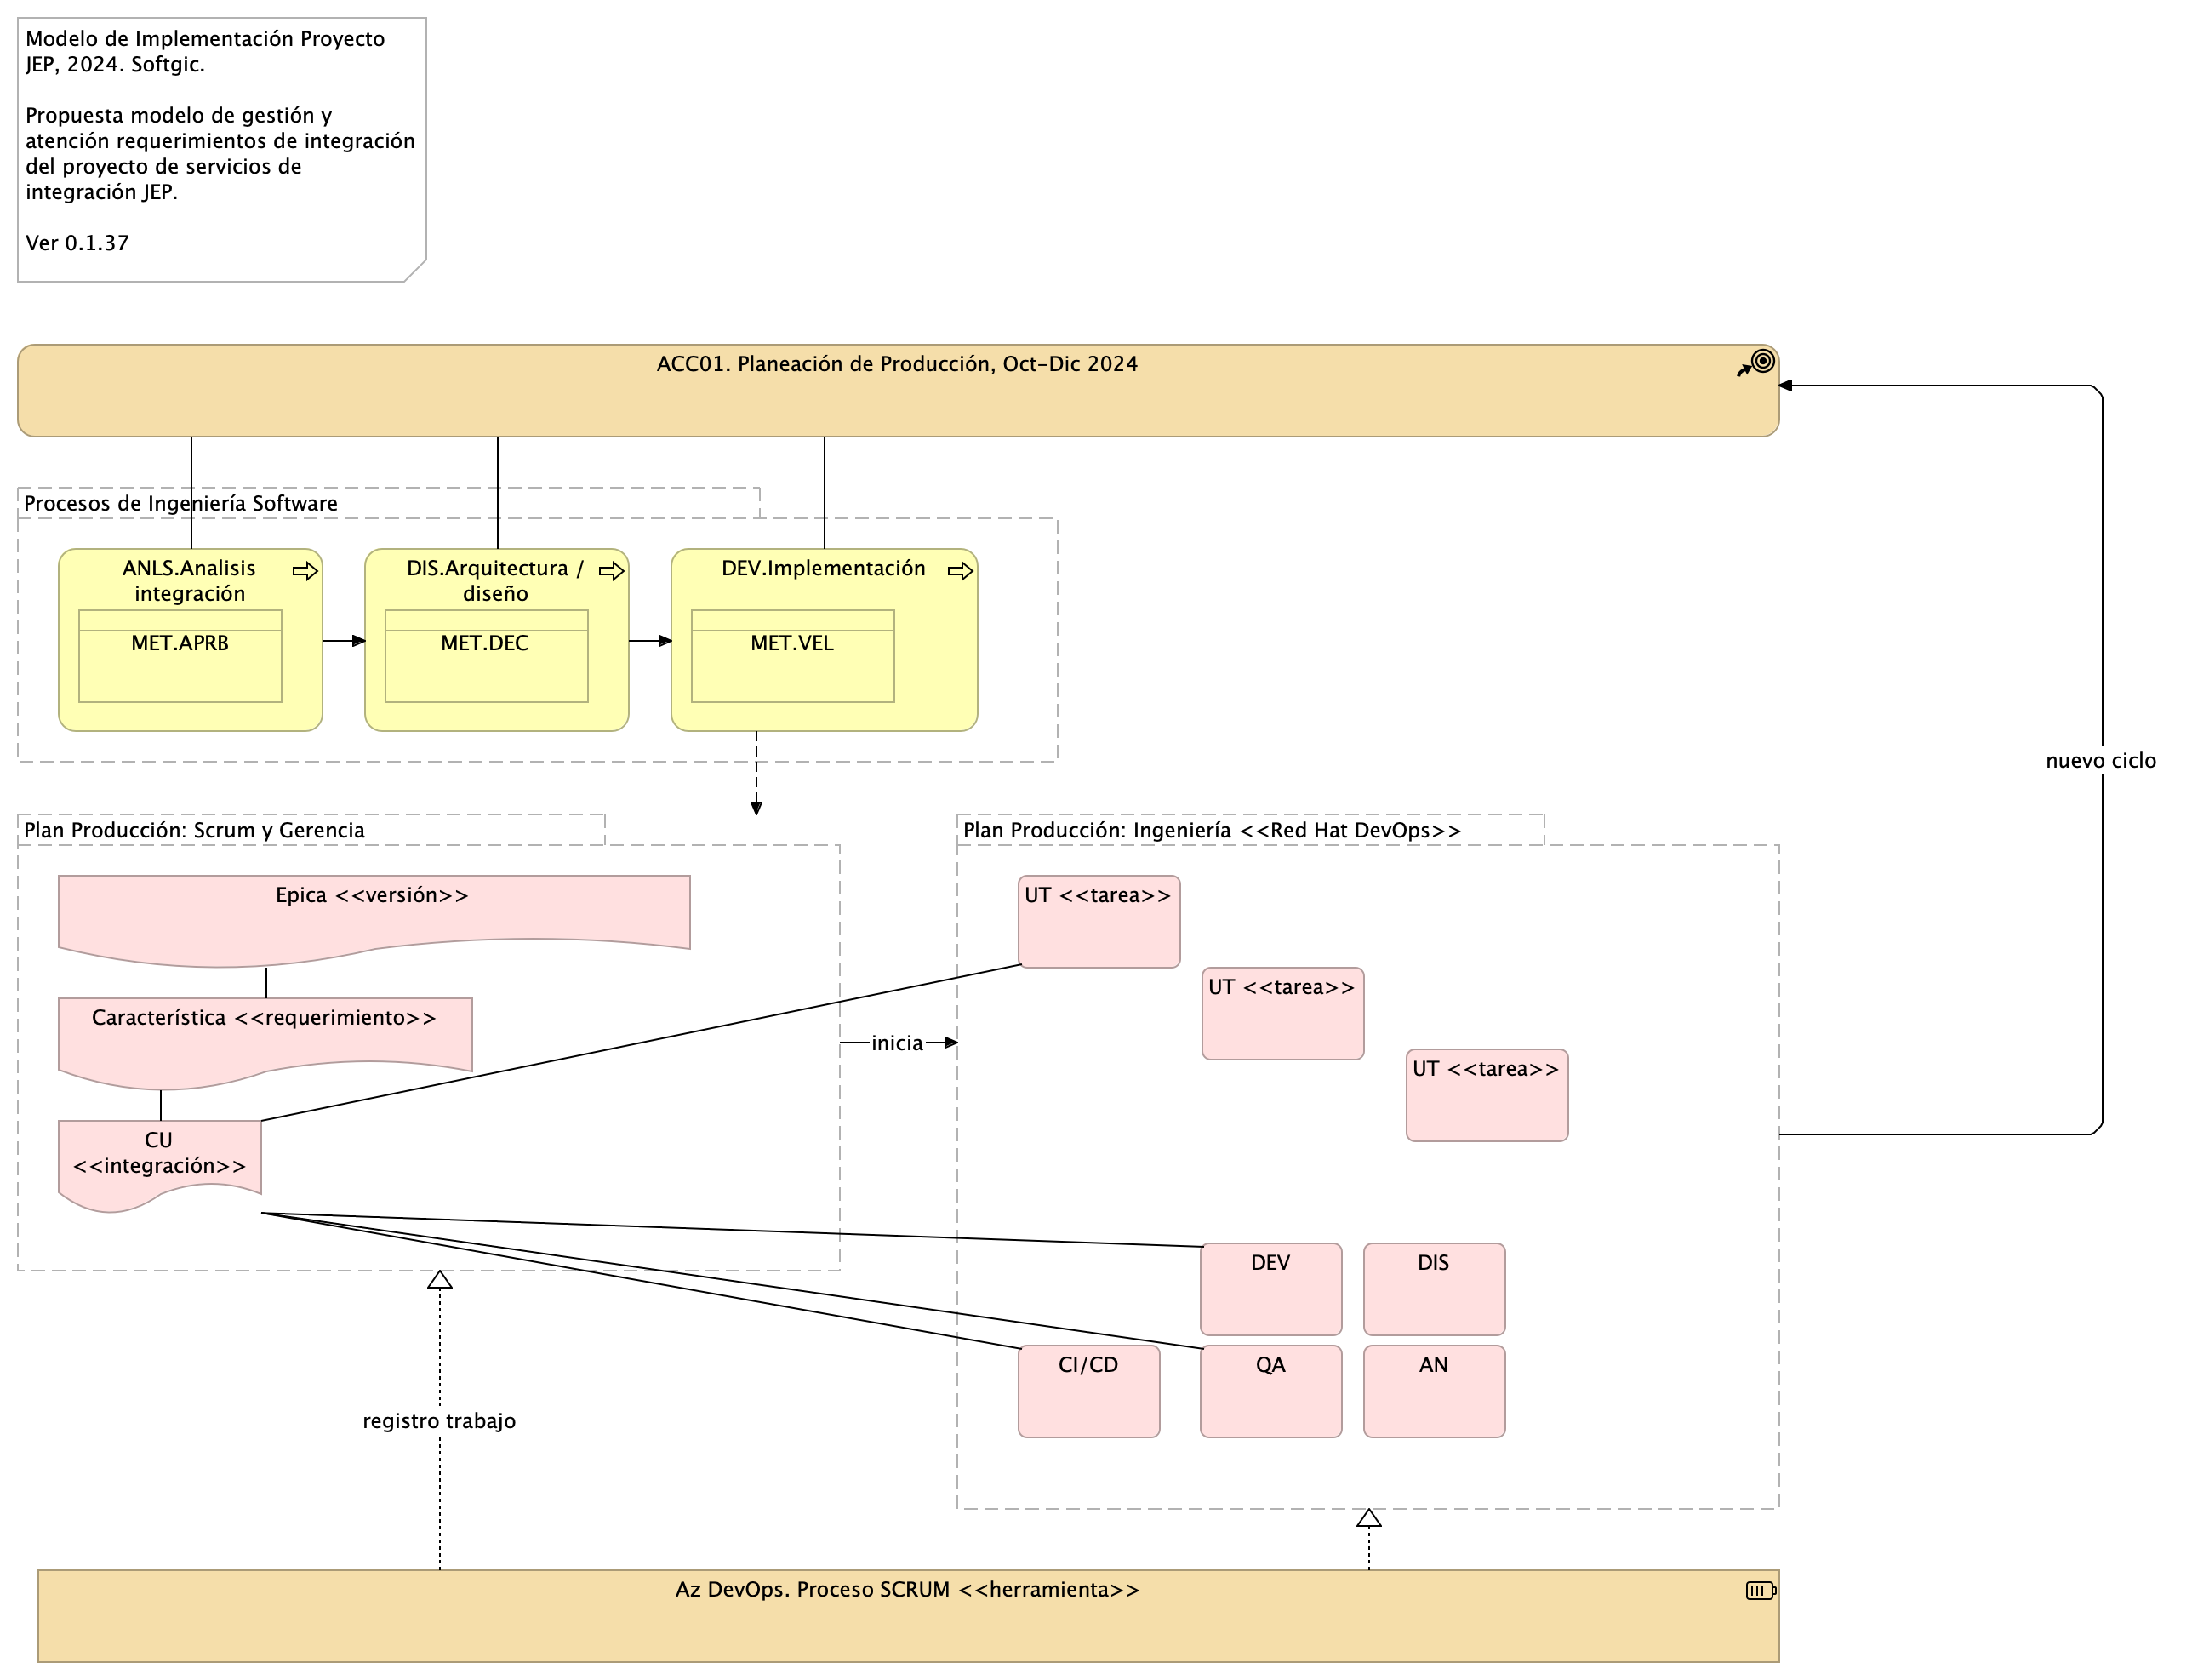
\includegraphics[width=\textwidth,height=5.20833in]{images/04.ING.2n.1a.Modelorequerimientos.png}
\caption{04.ING.2n.1a. Modelo requerimientos. \emph{Fuente: Repositorio
arquitectura Integración JEP
(2024)}}\label{fig:id-7c3abdaa8d9b46eebfd8f8e3e8d912ce}
\end{figure}

\subsubsection{Catálogo de
Elementos}\label{sec:catuxe1logo-de-elementos-1}

\begin{itemize}
\item
  \textbf{ACC01. Planeación de Producción, Oct-Dic 2024}. Objetivos y
  entregas en el tiempo, versiones de entrega del proyecto de
  integración.
\item
  \textbf{ANLS.Analisis integración}. \#\#\# 2. ANSS (análisis).
\item
  Scrum, Funcional, Dueño producto cliente (requiere conocimiento del
  negocio).
\item
  Resultado: Refinamiento HU, modelo de negocio, es decir, diagrama de
  HU relacionadas unas con otras y con los conceptos de negocio en el
  repositorio de ARQ. Actualmente: no hay resultados de este proceso.
  Ejemplo del modelo de negocio
\end{itemize}

\subsubsection{Salidas}\label{sec:salidas}

\begin{itemize}
\tightlist
\item
  Modelo de negocio en el repo
\item
  Estimación --puede en devops
\item
  Análisis de dependencia en el repo
\end{itemize}

\subsubsection{KPI}\label{sec:kpi}

\begin{itemize}
\item
  Tasa de aprobación de HU por cliente Fuente: (Cantidad de HU refinadas
  y aprobadas por cliente {[}Repo Sharepoint{]} / Total de cantidad de
  HU {[}Azure DevOps{]}) Dato 26/10/2023: (30/44) = 0,68
\item
  Tasa de error en Bug por PR entregados Fuente: (Cantidad de solicitude
  de cambio en rama (Pull Reqst) de Correcciones (fix) o Regresión
  (reverts) {[}Bitbucket{]} / Cantidad total de PR desplegados
  {[}Bitbucket{]}) Dato 26/10/2023: (8/111)*100 = 7,2\%
\item
  \textbf{CI/CD}. Actividades DevOps del ciclo o iteración de
  implementación.
\item
  \textbf{DEV}. Alcance de QA unitaria
\item
  \textbf{DEV.Implementación}. \#\#\# KPI
\item
  Velocidad de construcción Fuente: (Cantidad de puntos de HU ejecutadas
  {[}Azure DevOps{]} / Horas habiles del mes de trabajo {[}Calculo
  manual{]}) Dato 26/10/2023: 83 / 153 = 0,54 HU/horas
\item
  Tasa de cierre de defectos Fuente: (Cantidad de Bug solucionados
  {[}Azure DevOps{]} / Total de Bugs a corte sin nuevos {[}Azure
  DevOps{]}) Dato 26/10/2023: 81 / 920 = 0,088
\item
  Indice de dependecia de Lider Técnico Fuente: (Cantidad de actividades
  retrazadas semanales segun las HU planeadas / Total de HU planeadas
  para ejecución) Dato 26/10/2023: Pendiente proxima semana
\item
  \textbf{DIS.Arquitectura / diseño}. \#\#\# KPI
\item
  Nivel de HU sin detalle técnico Fuente: (Cantidad de HU refinadas y
  aprobadas sin diseño de implementacion {[}Repo Sharepoint{]} / Total
  de cantidad de HU {[}Azure DevOps{]}) Dato 26/10/2023: 0/44=0
\item
  \textbf{MET.APRB}. Cod. APRB Nombre indicador Tasa de aprobación de HU
  por cliente Uso Estabildad de requerimientos. Contensión del flujo de
  trabajo inicio de desarrolo Proceso ANLS Calculo de medición Cantidad
  de HU refinadas y aprobadas por cliente / Total de cantidad de HU
  Fuente {[}Repo Sharepoint{]}, {[}Azure DevOps{]})
\item
  \textbf{MET.DEC}. Cod.: DEC Nombre indicador: Decisiones de diseño,
  justificaciones, validaciones Uso: Estabildad de requerimientos.
  Control de alineación desarrollo-demanda Proceso: DIS Calculo de
  medición: Cantidad de HU refinadas y aprobadas por cliente / Total de
  cantidad de HU Fuente: {[}Repo Sharepoint{]}, {[}Azure DevOps{]})
\item
  \textbf{MET.VEL}. Cod. VEL Nombre indicador Velocidad de construcción
  Uso Capacidad interna de desarrollo Proceso DEV Calculo de medición
  Cantidad de puntos de HU ejecutadas / Horas habiles del mes de trabajo
  Fuente {[}Azure DevOps{]}, {[}Calculo manual{]}
\item
  \textbf{UT (tarea)}. Unidad mínima de trabajo (tarea por
  desarrollador).
\end{itemize}

\newpage

\section{Modelo de Producción e
Implementación}\label{sec:modelo-de-producciuxf3n-e-implementaciuxf3n}

\subsection{Modelo de Producción e Implementación de Integración
JEP}\label{sec:modelo-de-producciuxf3n-e-implementaciuxf3n-de-integraciuxf3n-jep}

\begin{quote}
Modelo de Producción e Implementación Proyecto JEP, 2024. Softgic.
Modelo de gestión y atención requerimientos de integración del proyecto
de integración JEP, 2024. Softgic. Relación con herramienta de gestión
Az DevOps. Ver 0.1.12
\end{quote}

El modelo de producción que procesa los requerimientos del proyecto JEP
inicia con la creación de un tramo de la planeación de la solución de
integración, esto es un ciclo de implementación o iteración del proyecto
de integración JEP.

(ING) Procesos de ingeniería. Arrancan los procesos mínimos de
ingeniería previos a la construcción de la integración.

(PRY) Planificación de historias de usuario. La porción de la planeación
de producción aprobada para la construcción se planifica en historias o
casos de uso, u cualquier otra forma de medición de avance.

(ING) Creación e inicio de iteraciones de implementación incremental. La
planificación de HU (CU, u otra) es tareificada y asignada a
desarrolladores disponibles. Además, las tareas asignadas son
organizadas en ciclos de trabajo fijo (iteraciones). Esta ejecución es
la línea de trabajo principal del proyecto JEP.

(PRY, ING) Coordinación de líneas de trabajo. Las entregas de la línea
de trabajo del proyecto JEP debe ser compasada con otras líneas de
trabajo de la JEP, con las que puede haber una relación de secuencia o
dependencia externa.

Durante la ejecución de la iteraciones determinadas, inicia nuevamente
el ciclo del proyecto desde la creación de un nuevo tramo de la
planeación de producción.

\subsubsection{Mapeo del Modelo con Herramienta de Registro del Trabajo
(az
devops)}\label{sec:mapeo-del-modelo-con-herramienta-de-registro-del-trabajo-az-devops}

\begin{itemize}
\tightlist
\item
  Épica = Versión de entrega de la solución como un todo
\item
  Característica = Requerimiento de integración, del cual pueden
  desprenderse varias integraciones puntuales.
\item
  HU = Una integración puntual proveniente de un requerimiento, ej.:
  ingreso Conti, Consulta campos, Radicar ítem, Generación
  documentos\ldots{}
\item
  UT = Tarea de desarrollo.
\end{itemize}

\begin{figure}
\centering
\includegraphics[width=\textwidth,height=5.20833in]{images/04.ING.2n.1b.Modeloproducción.png}
\caption{04.ING.2n.1b. Modelo producción. \emph{Fuente: Repositorio
arquitectura Integración JEP
(2024)}}\label{fig:id-9938d5859d53450fa5c5c953d9ce33cb}
\end{figure}

\subsubsection{Catálogo de
Elementos}\label{sec:catuxe1logo-de-elementos-2}

\begin{longtable}[]{@{}
  >{\raggedright\arraybackslash}p{(\columnwidth - 4\tabcolsep) * \real{0.3000}}
  >{\raggedright\arraybackslash}p{(\columnwidth - 4\tabcolsep) * \real{0.2000}}
  >{\raggedright\arraybackslash}p{(\columnwidth - 4\tabcolsep) * \real{0.5000}}@{}}
\toprule\noalign{}
\begin{minipage}[b]{\linewidth}\raggedright
Nombre
\end{minipage} & \begin{minipage}[b]{\linewidth}\raggedright
Tipo
\end{minipage} & \begin{minipage}[b]{\linewidth}\raggedright
Documentación
\end{minipage} \\
\midrule\noalign{}
\endhead
\bottomrule\noalign{}
\endlastfoot
ACC01. Planeación de Producción, Oct-Dic 2024 & Course Of-Action &
Objetivos y entregas en el tiempo, versiones de entrega del proyecto de
integración. \\
& & \\
ANLS.Analisis integración & Business Process & \#\#\# 2. ANSS
(análisis). \\
\end{longtable}

\begin{itemize}
\tightlist
\item
  Scrum, Funcional, Dueño producto cliente (requiere conocimiento del
  negocio).
\item
  Resultado: Refinamiento HU, modelo de negocio, es decir, diagrama de
  HU relacionadas unas con otras y con los conceptos de negocio en el
  repositorio de ARQ. Actualmente: no hay resultados de este proceso.
  Ejemplo del modelo de negocio
\end{itemize}

\subsubsection{Salidas}\label{sec:salidas-1}

\begin{itemize}
\tightlist
\item
  Modelo de negocio en el repo
\item
  Estimación --puede en devops
\item
  Análisis de dependencia en el repo
\end{itemize}

\subsubsection{KPI}\label{sec:kpi-1}

\begin{itemize}
\item
  Tasa de aprobación de HU por cliente Fuente: (Cantidad de HU refinadas
  y aprobadas por cliente {[}Repo Sharepoint{]} / Total de cantidad de
  HU {[}Azure DevOps{]}) Dato 26/10/2023: (30/44) = 0,68
\item
  Tasa de error en Bug por PR entregados Fuente: (Cantidad de solicitude
  de cambio en rama (Pull Reqst) de Correcciones (fix) o Regresión
  (reverts) {[}Bitbucket{]} / Cantidad total de PR desplegados
  {[}Bitbucket{]}) Dato 26/10/2023: (8/111)*100 = 7,2\% \textbar{}
  \textbar{} CI/CD \textbar{} Work Package \textbar{} Actividades DevOps
  del ciclo o iteración de implementación. \textbar{} \textbar{} DEV
  \textbar{} Work Package \textbar{} Alcance de QA unitaria \textbar{}
  \textbar{} DEV \textbar{} Work Package \textbar{} Alcance de QA
  unitaria \textbar{} \textbar{} DEV.Implementación \textbar{} Business
  Process \textbar{} \#\#\# KPI
\item
  Velocidad de construcción Fuente: (Cantidad de puntos de HU ejecutadas
  {[}Azure DevOps{]} / Horas habiles del mes de trabajo {[}Calculo
  manual{]}) Dato 26/10/2023: 83 / 153 = 0,54 HU/horas
\item
  Tasa de cierre de defectos Fuente: (Cantidad de Bug solucionados
  {[}Azure DevOps{]} / Total de Bugs a corte sin nuevos {[}Azure
  DevOps{]}) Dato 26/10/2023: 81 / 920 = 0,088
\item
  Indice de dependecia de Lider Técnico Fuente: (Cantidad de actividades
  retrazadas semanales segun las HU planeadas / Total de HU planeadas
  para ejecución) Dato 26/10/2023: Pendiente proxima semana \textbar{}
  \textbar{} DIS.Arquitectura / diseño \textbar{} Business Process
  \textbar{} \#\#\# KPI
\item
  Nivel de HU sin detalle técnico Fuente: (Cantidad de HU refinadas y
  aprobadas sin diseño de implementacion {[}Repo Sharepoint{]} / Total
  de cantidad de HU {[}Azure DevOps{]}) Dato 26/10/2023: 0/44=0
  \textbar{} \textbar{} MET.APRB \textbar{} Business Object \textbar{}
  Cod. APRB Nombre indicador Tasa de aprobación de HU por cliente Uso
  Estabildad de requerimientos. Contensión del flujo de trabajo inicio
  de desarrolo Proceso ANLS Calculo de medición Cantidad de HU refinadas
  y aprobadas por cliente / Total de cantidad de HU Fuente {[}Repo
  Sharepoint{]}, {[}Azure DevOps{]}) \textbar{} \textbar{} MET.DEC
  \textbar{} Business Object \textbar{} Cod.: DEC Nombre indicador:
  Decisiones de diseño, justificaciones, validaciones Uso: Estabildad de
  requerimientos. Control de alineación desarrollo-demanda Proceso: DIS
  Calculo de medición: Cantidad de HU refinadas y aprobadas por cliente
  / Total de cantidad de HU Fuente: {[}Repo Sharepoint{]}, {[}Azure
  DevOps{]})
\end{itemize}

\textbar{} \textbar{} MET.VEL \textbar{} Business Object \textbar{} Cod.
VEL Nombre indicador Velocidad de construcción Uso Capacidad interna de
desarrollo Proceso DEV Calculo de medición Cantidad de puntos de HU
ejecutadas / Horas habiles del mes de trabajo Fuente {[}Azure DevOps{]},
{[}Calculo manual{]} \textbar{} \textbar{} UT (tarea) \textbar{} Work
Package \textbar{} Unidad mínima de trabajo (tarea por desarrollador).
\textbar{}

Table: Elementos de la vista.
\{\#tbl:tblelement-04.ING.2n.1b.Modeloproducción-id\}

\newpage

\section{Modelo de Solución de
Interoperabilidad}\label{sec:modelo-de-soluciuxf3n-de-interoperabilidad}

\subsection{Modelo de Interoperabilidad
JEP}\label{sec:modelo-de-interoperabilidad-jep}

\begin{quote}
Modelo de Integración. Proyecto JEP, 2024. Softgic. Capacidades del
modelo de integración para la implementación de requerimientos de
interoperabilidad del proyecto Integración JEP, 2024. Ver 0.2.44
\end{quote}

El presente modelo de solución de interoperabilidad JEP, 2024, en
desarrollo por Softgic, expone para aprobación y referencia las
decisiones de la solución de integración y las restricciones que la
rigen. Una vez revisado y aprobado por parte de JEP el modelo de
interoperabilidad será referencia para la gestión del proyecto y de los
entregables de esta solución.

\subsection{Características Principales del Modelo de Integración
JEP}\label{sec:caracteruxedsticas-principales-del-modelo-de-integraciuxf3n-jep}

\begin{itemize}
\tightlist
\item
  API de integración
\item
  Patrones de integración empresarial (EIP)
\item
  Sistema de Mensajería entre servicios de integración y aplicaciones
  JEP
\item
  Flujos de datos para integración
\item
  Arquitectura de clusters y contenedores para integración
\item
  Uso de infraestructura tecnológica JEP
\item
  Articulación con el Service Mesh de JEP
\end{itemize}

\begin{figure}
\centering
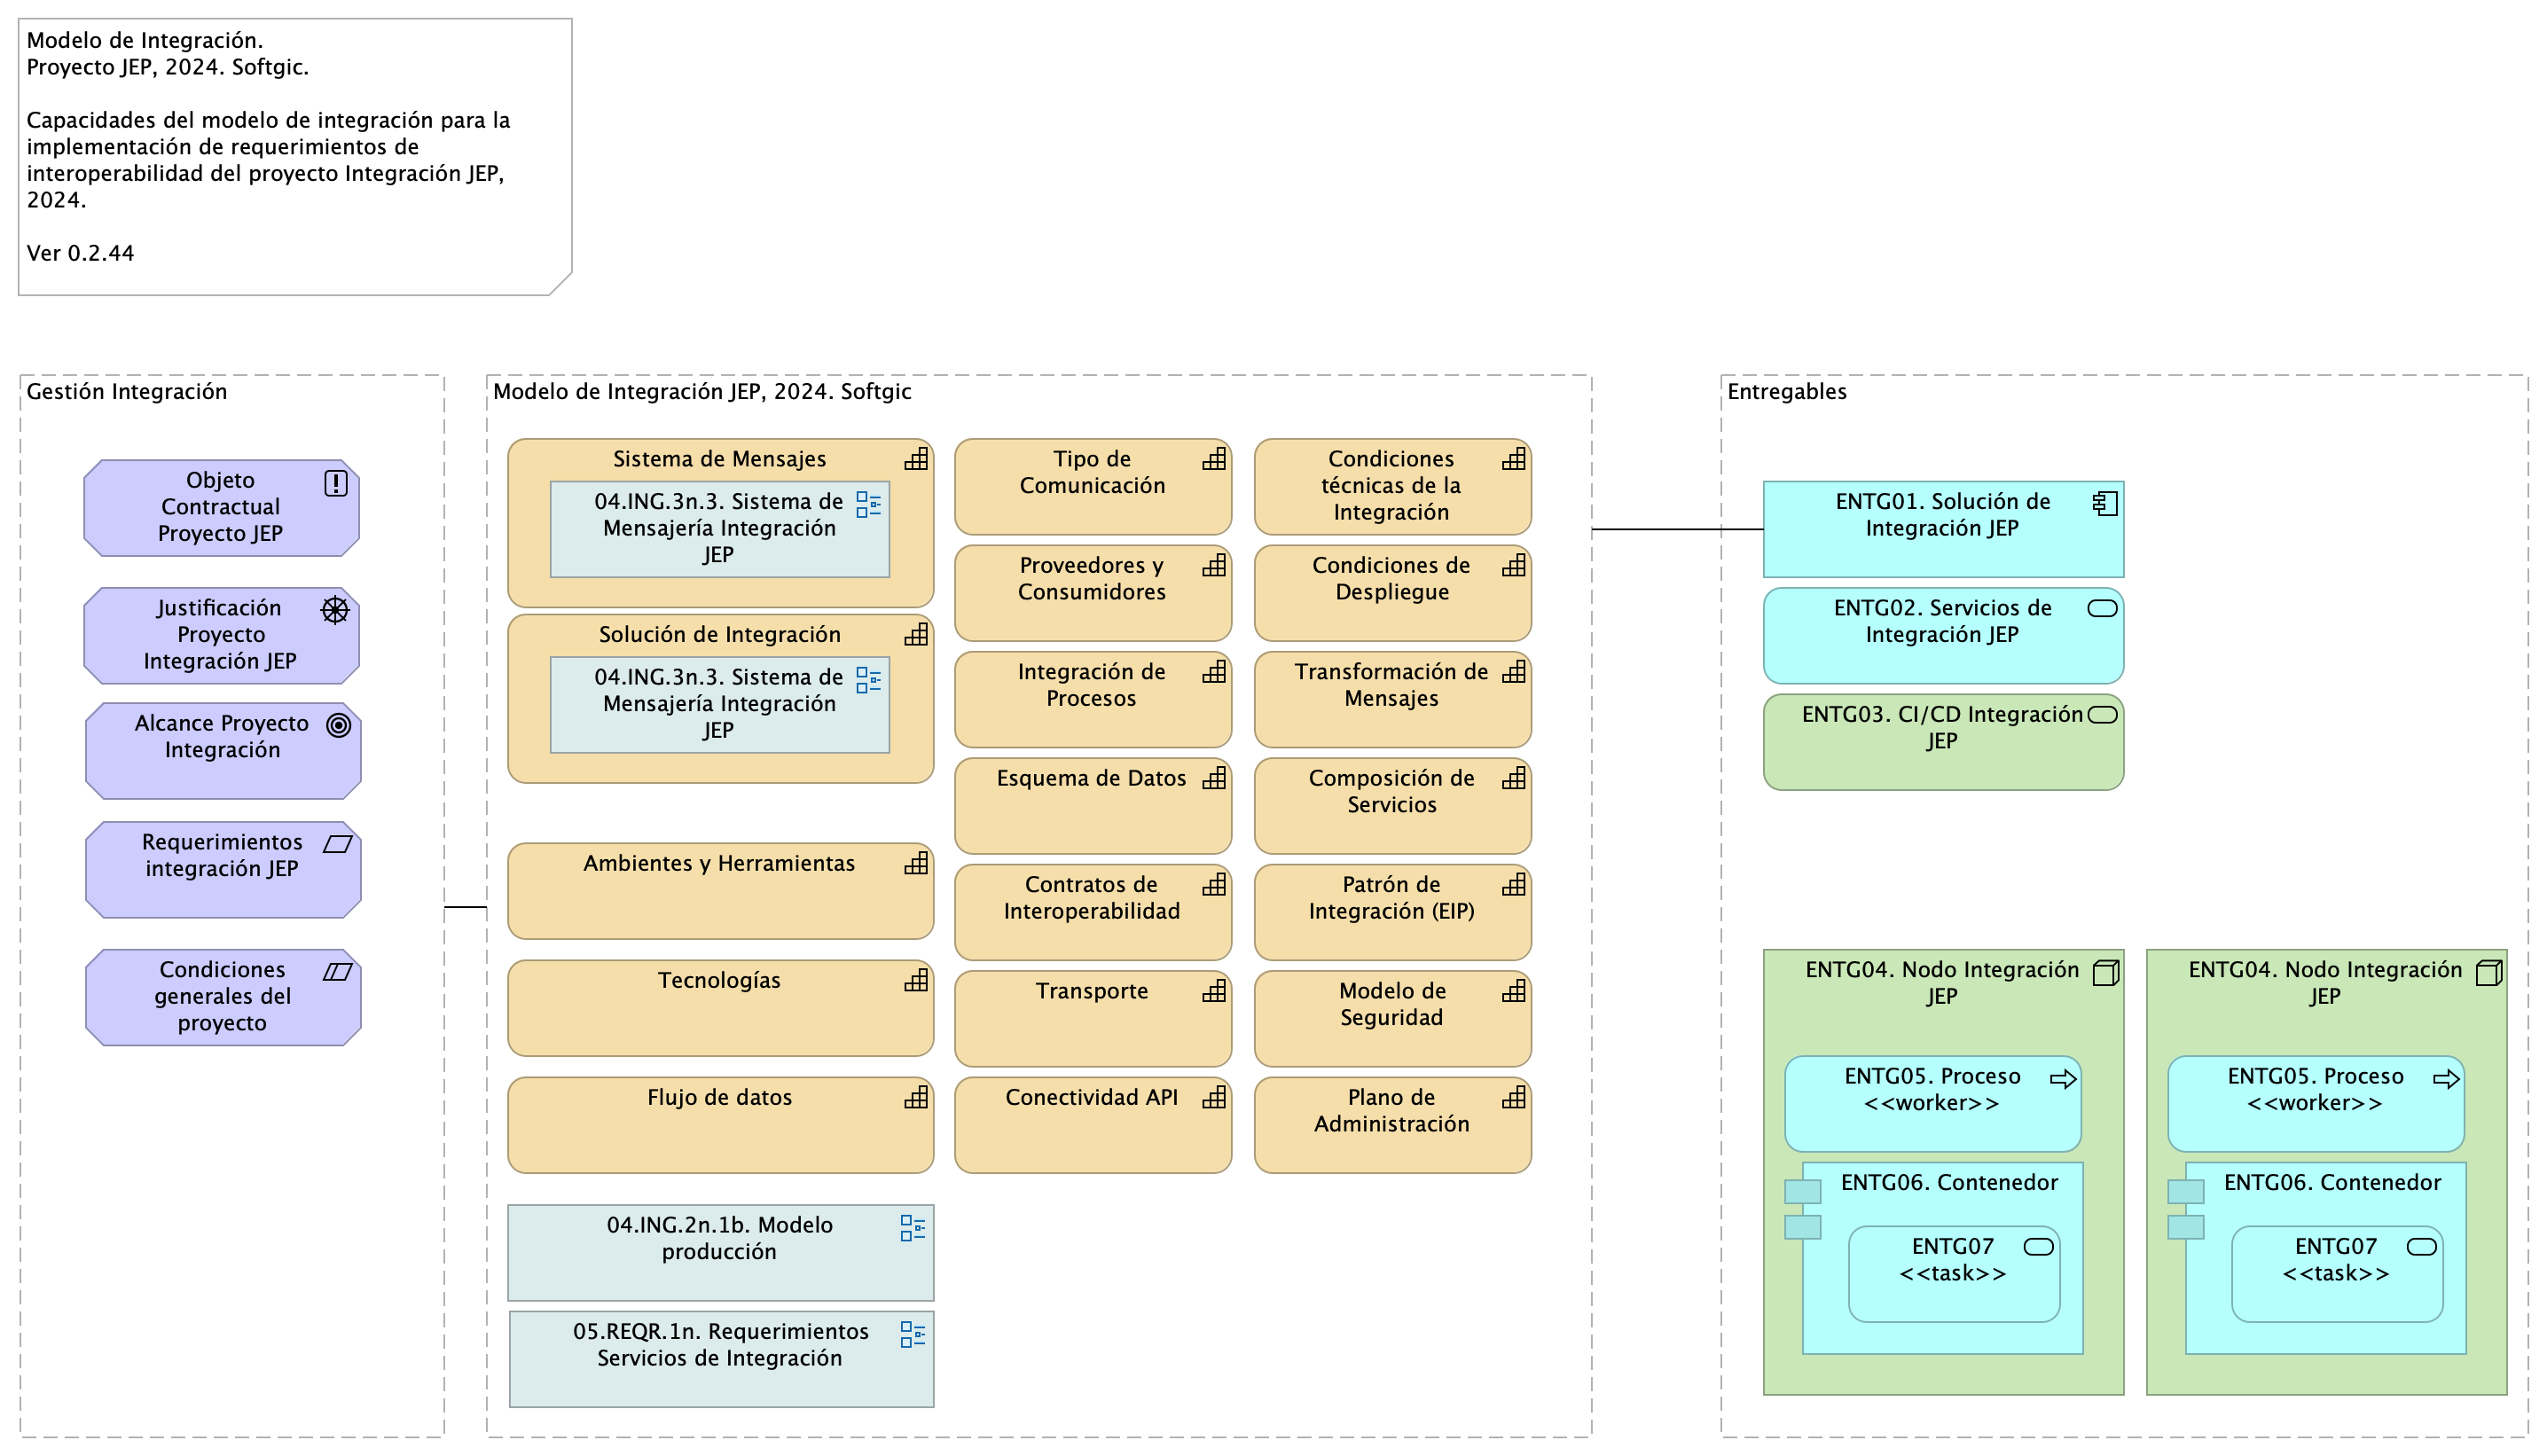
\includegraphics[width=\textwidth,height=5.20833in]{images/04.ING.3n.1.ModelodeInteroperabilidadJEP.png}
\caption{04.ING.3n.1. Modelo de Interoperabilidad JEP. \emph{Fuente:
Repositorio arquitectura Integración JEP
(2024)}}\label{fig:id-f863abde3ea94046a77bf84d5cb0a3a8}
\end{figure}

\subsubsection{Catálogo de
Elementos}\label{sec:catuxe1logo-de-elementos-3}

\begin{longtable}[]{@{}lll@{}}
\toprule\noalign{}
Nombre & Tipo & Documentación \\
\midrule\noalign{}
\endhead
\bottomrule\noalign{}
\endlastfoot
Alcance Proyecto Integración & Goal & Es del alcance del proyecto \\
\end{longtable}

\begin{enumerate}
\def\labelenumi{\arabic{enumi}.}
\tightlist
\item
  Implementación de 20 o más servicios de integración al 31 de diciembre
  del 2024.
\item
  Soporte solución de integración a julio 2025.
\end{enumerate}

No es del alcance del proyecto el desarrollo a la medida de soluciones
de las aplicaciones y sistemas de software de la JEP.

No es del alcance de este proyecto los requerimientos de migración de
los servicios de integración existentes de la JEP (hayan sido o no
implementados bajo el modelo integración directa --EIA).

\textbar{} \textbar{} Ambientes y Herramientas \textbar{} Capability
\textbar{} Esta solución de interoperabilidad usa las herramientas,
librerías, ambientes, infraestructura productivo y no productivos
(nodos, redes, almacenamientos, y otros) indicados por la JEP.
\textbar{} \textbar{} Composición de Servicios \textbar{} Capability
\textbar{} Combina colección de servicios para formar un servicio
completo. Mediante la integración basada en patrones de Camel, define
funciones mediante la recopilación de datos de múltiples conexiones
(endpoint). Las composiciones suelen resolver integraciones no triviales
o complejas. \textbar{} \textbar{} Condiciones generales del proyecto
\textbar{} Constraint \textbar{} Son condiciones generales de la
solución aquellas que inciden en la gestión del proyecto, entrega de
productos contractuales y el desarrollo del software de integración, las
siguientes:

\begin{enumerate}
\def\labelenumi{\arabic{enumi}.}
\tightlist
\item
  Las integraciones provistas por esta solución son unidades ejecutables
  desplegables entendidas como servicios de integración directamente
  relacionados con las historias de usuario, y éstas se corresponden con
  los servicios indicados en el alcance contractual del proyecto:
  ``Implementación de 20 o más servicios de integración al 31 de
  diciembre del 2024''. Dicho de otra manera, los servicios de
  integración de esta solución son a la vez historias de usuario, y
  servicios de alcance del proyecto.
\item
  Un servicio de integración de esta solución es un entregable de
  software que involucra a aplicaciones consumidoras y proveedoras, y
  contiene mensaje de interacción, un intermediador de mensajes, ej. un
  bus de integración, y una o más operaciones de integración
  empresarial.
\item
  Los servicios de integración de esta solución (servicios del alcance
  según el numeral anterior) no se extiende al cambio de las reglas de
  negocio de la JEP, ni a sus aplicaciones que las ejecuten. Únicamente
  se limita a realizar operaciones de integración sobre las capacidades
  existentes de las aplicaciones.
\item
  Para efectos de mantener la continuidad de las entregas, sin
  perjudicar ni a la calidad, ni a la aceptación de esta solución de
  integración, aquellas capacidades de las aplicaciones de software de
  la JEP que generen depedencias o que no estén disponibles al momento
  del desarrollo de los servicios de integración de esta solución serán
  provitas por Softgic y funcionarán como sustitutas equivalentes.
\end{enumerate}

Estas condiciones generales deben ser observadas e informadas a todas
las partes. \textbar{} \textbar{} Condiciones técnicas de la Integración
\textbar{} Capability \textbar{} * Uso de infraestructura,
almacenamiento y cómputo de la JEP: Openshift Platform, bus empresarial,
seguridad de la empresa, tecnoglogía de clusters y contenedores, y
Prometheus como la herramienta de monitoreo de servicios.

\begin{itemize}
\item
  Monitoreo de uso de los recursos de procesamiento, red y memoria de
  los componentes claves de la solución haciendo uso de ServiceMesh.
\item
  La solución soporta la habilitación de reglas de alertas sobre los
  registros de actividad y monitoreo.
\item
  Soluciones de EFK (Elasticsearch, FluentD, Kibana - ELKstack), a
  través de operadores para centralizar el proceso de logs que se
  generan en difrerentes espacios de trabajo.
\end{itemize}

Estas condiciones técnicas y tecnológicas deben ser observadas e
informadas a todas las partes. \textbar{} \textbar{} Conectividad API
\textbar{} Capability \textbar{} Esta solución de interoperabilidad usa
conectividad API REST provista por la infraestructura de conectividad de
la JEP (Apache Camel). \textbar{} \textbar{} ENTG01. Solución de
Integración JEP \textbar{} Application Component \textbar{}
Documentación técnica del diseño de solución de la integración JEP,
2024. \textbar{} \textbar{} ENTG02. Servicios de Integración JEP
\textbar{} Application Service \textbar{} Servicios ejecutables
desplegados en los entornos de software JEP. \textbar{} \textbar{}
ENTG03. CI/CD Integración JEP \textbar{} Technology Service \textbar{}
Cadenas de integración y despliegue continuo de los servicios de
integración del proyecto de integración JEP, 2024. \textbar{} \textbar{}
ENTG04. Nodo Integración JEP \textbar{} Node \textbar{} Cluster de
ejecución de los nodos y procesos de (servicios) de integración del
proyecto. \textbar{} \textbar{} ENTG05. Proceso (worker) \textbar{}
Application Process \textbar{} Configuración de servicios de integración
del proyecto dentro de la infraestructura tecnológica JEP. \textbar{}
\textbar{} ENTG06. Contenedor \textbar{} Application Component
\textbar{} Contenedores de los servicios de integración del proyecto
desplegados en la infraestructura tecnológica JEP. \textbar{} \textbar{}
ENTG07 (task) \textbar{} Application Service \textbar{} Servicios de
integración del proyecto desplegados en la infraestructura tecnológica
JEP. \textbar{} \textbar{} Flujo de datos \textbar{} Capability
\textbar{} Esta solución de interoperabilidad usa esquemas de datos
predefinidos entre las integraciones. \textbar{} \textbar{}
Justificación Proyecto Integración JEP \textbar{} Driver \textbar{}
Justificación Proyecto Integración JEP \textbar{} Driver \textbar{}
Justification: Evolución de la Plataforma de Interoperabilidad para el
ano 2024

\begin{enumerate}
\def\labelenumi{\arabic{enumi}.}
\tightlist
\item
  Evolución de la plataforma tecnología de su interoperabilidad y el
  cumplimiento de los lineamientos del MinTIC, a traves del ``Manual
  Interactivo de Gobierno Digital, herramienta dirigida a las entidades
  publicas nacionales y territoriales (\ldots) Política de Gobierno
  Digital, Decreto 767 de 2022''
\item
  Interoperabilidad con las entidades externas que demandan información
  de la JEP
\item
  Evolución del modelo de interoperabilidad interna y gobierno de data
  maestra entre sistemas internos \textbar{} \textbar{} Modelo de
  Seguridad \textbar{} Capability \textbar{} Autenticación mixta: JWS y
  tradicional (usuario, contraseña). \textbar{} \textbar{} Objeto
  Contractual Proyecto JEP \textbar{} Principle \textbar{} Prestar los
  servicios de administración y monitoreo de la solución de
  interoperabilidad de los sistemas de información de la JEP; así como
  la implementación de nuevos desarrollos o parametrizaciones que esta
  solución requiera. \textbar{} \textbar{} Patrón de Integración (EIP)
  \textbar{} Capability \textbar{} Pasar de modelo integración EIA
  (intgración directa ente consumidores y proveedores) a modelo de
  integración EIP (integración empresarial/bus) sobre Red Hat
  Integration Platform.
\end{enumerate}

\textbar{} \textbar{} Plano de Administración \textbar{} Capability
\textbar{} Monitoreo de rendimiento de ssvc de integración. \textbar{}
\textbar{} Requerimientos integración JEP \textbar{} Requirement
\textbar{} Del alcance del proyecto,

\begin{enumerate}
\def\labelenumi{\arabic{enumi}.}
\tightlist
\item
  Implementación de 20 o más servicios de integración al 31 de diciembre
  del 2024.
\item
  Soporte solución de integración a julio 2025.
\end{enumerate}

Establecemos las bases para el modelo de requerimientos de esta
solución, el cual limita la demana a:

\begin{itemize}
\tightlist
\item
  Desarrollar únicamente nuevos servicios de integración con el patrón
  de integración empresarial (ESB, Camel K de Apache) propuesto en el
  modelo de interoperabilidad de esta solución.
\item
  Implementar en esta solución de integración las condiciones
  tecnológicas JEP, entendidas como requerimientos no funcionales de
  arquitectura, presentes en el Anexo Nro. 1.1 -- Anexo técnico
  evolución plataforma de interoperabilidad -- Ficha Técnica.
\item
  No son requerimientos de este proyecto el implementar otro tipos de
  requerimientos no expresados aquí, como por ejemplo, migrar los
  servicios existentes de modelo integración directa (EIA) esta solución
  de integración empresarial, o implementar soluciones en las
  aplicaciones de software de la JEP. \textbar{} \textbar{} Sistema de
  Mensajes \textbar{} Capability \textbar{} Esta solución de
  interoperabilidad usa un sistema de mensajes (comandos). Los mensajes
  son de tipo petición, respuesta o excepción.
\end{itemize}

La mensajería puede ser asíncrona o síncrona entre aplicaciones o
servicios desacoplados. La conexión y la sesión es manejada por un
agente intermediario, que puede ser una cola o un bus empresarial (para
este contexto, OpenShift, Cliente Red Had Interoperabity o Apache
Camel).

La comunicación del sistema de mensajería ocurre cuando la aplicación o
servicio productor emite un comando (mensaje ) de `envío', en el cual
transmite datos o peticiones de negocio en un formato predefinido, y lo
envía a una cola de mensajes. \textbar{} \textbar{} Solución de
Integración \textbar{} Capability \textbar{} Estilos de Integración:
Communications backbone \footnote{Red troncal de comunicaciones: a
  medida que más y más aplicaciones de una empresa se conectan al
  sistema de mensajería y hacen que su funcionalidad esté disponible a
  través de la mensajería, el sistema de mensajería se convierte en un
  punto centralizado de ventanilla única para la funcionalidad en la
  empresa. Una nueva aplicación simplemente necesita saber qué canales
  usar para solicitar funcionalidad y cuáles otros escuchar para obtener
  los resultados. El propio sistema de mensajería se convierte
  esencialmente en un bus de mensajes, una columna vertebral que
  proporciona acceso a todas las diversas y cambiantes aplicaciones y
  funcionalidades de la empresa. Puedes lograr este nirvana de
  integración más rápida y fácilmente si diseñas específicamente para
  ello desde el principio. \textbar{} \textbar{} Tecnologías \textbar{}
  Capability \textbar{} * Red Hat Integration: suite de runtimes,
  frameworks, y servicios para aplicaciones nativas de Red Hat
  OpenShift. * Camel Integration Tool * Quarkus development framework *
  Java OpenJDK 17 * EFK (Elasticsearch, FluentD, Kibana - ELKstack)
  \textbar{} \textbar{} Tipo de Comunicación \textbar{} Capability
  \textbar{} Pasar llamadas síncronas a asincrónicas: analizar apps que
  deben cambiar comunicación \textbar{} \textbar{} Transformación de
  Mensajes \textbar{} Capability \textbar{} Mapeos, homologaciones y
  correspondencias. \textbar{}}. Patrón principal: Messaging --- Cada
aplicación (app) conectada a un mismo sistema de mensajería, intercambio
de datos y operación entre aplicaciones mediante mensajes.

Table: Elementos de la vista.
\{\#tbl:tblelement-04.ING.3n.1.ModelodeInteroperabilidadJEP-id\}

\subsection{Ambientes y Herramientas. Organización de Referencia
JEP}\label{sec:ambientes-y-herramientas.-organizaciuxf3n-de-referencia-jep}

Ambientes y Herramientas de Referencia JEP

\begin{quote}
Integraciones JEP, 2024 Integración JEP. Softgic. Ambientes y
Herramientas. Organización de referencia. versión 0.1.44
\end{quote}

Organización de referencia de los ambientes de trabajo JEP.

\begin{figure}
\centering
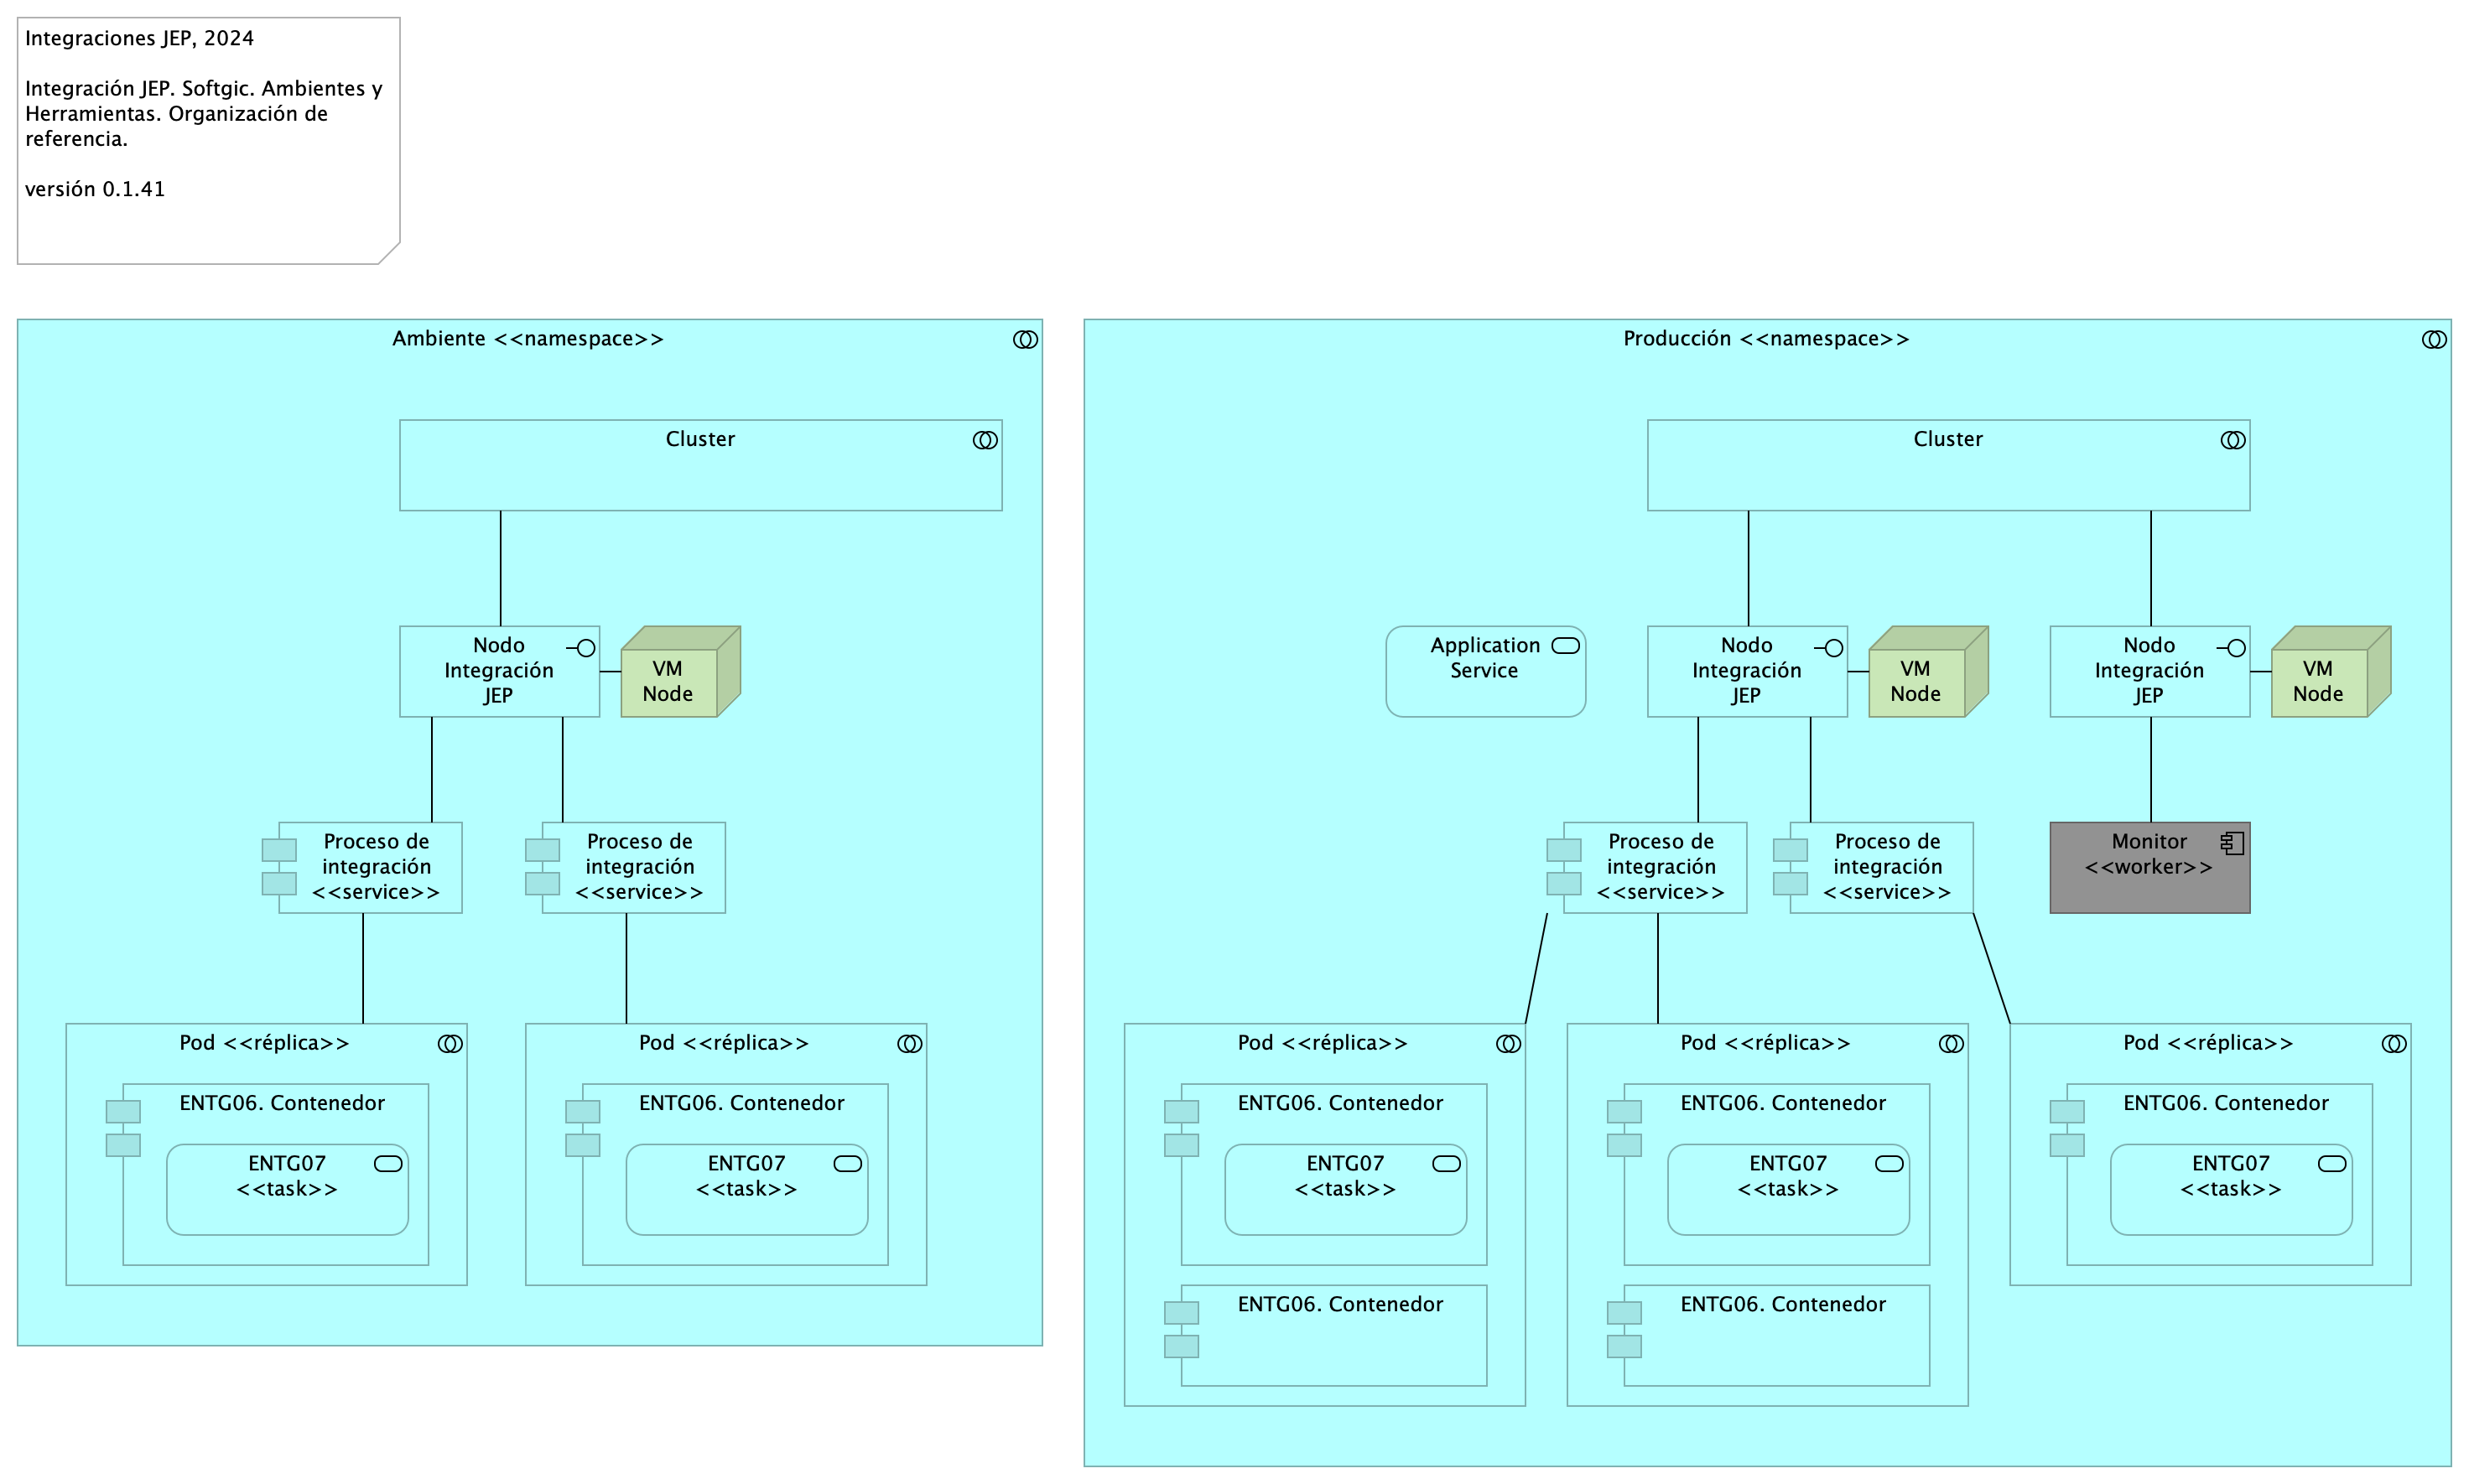
\includegraphics[width=\textwidth,height=5.20833in]{images/04.ING.3n.2.AmbientesyHerramientasJEP.png}
\caption{04.ING.3n.2. Ambientes y Herramientas JEP. \emph{Fuente:
Repositorio arquitectura Integración JEP
(2024)}}\label{fig:id-53af0cb1d4e145a6b82764f7ce8f9237}
\end{figure}

\subsubsection{Catálogo de
Elementos}\label{sec:catuxe1logo-de-elementos-4}

\begin{longtable}[]{@{}
  >{\raggedright\arraybackslash}p{(\columnwidth - 4\tabcolsep) * \real{0.3000}}
  >{\raggedright\arraybackslash}p{(\columnwidth - 4\tabcolsep) * \real{0.2000}}
  >{\raggedright\arraybackslash}p{(\columnwidth - 4\tabcolsep) * \real{0.5000}}@{}}
\toprule\noalign{}
\begin{minipage}[b]{\linewidth}\raggedright
Nombre
\end{minipage} & \begin{minipage}[b]{\linewidth}\raggedright
Tipo
\end{minipage} & \begin{minipage}[b]{\linewidth}\raggedright
Documentación
\end{minipage} \\
\midrule\noalign{}
\endhead
\bottomrule\noalign{}
\endlastfoot
Cluster & Application Collaboration & Orquestador de nodos y servicios
(contendores) de la JEP. \\
& & \\
ENTG06. Contenedor & Application Component & Contenedores de los
servicios de integración del proyecto desplegados en la infraestructura
tecnológica JEP. \\
& & \\
ENTG07 (task) & Application Service & Servicios de integración del
proyecto desplegados en la infraestructura tecnológica JEP. \\
& & \\
Nodo Integración JEP (worker) & Application Collaboration & Nodo lógico
en donde corren los contenedores. \\
& & \\
Proceso de integración (kb service) & Application Interface & Definición
de un proceso de trabajo de integración desplegable. \\
\end{longtable}

\textbar{} \textbar{} VM Node \textbar{} Node \textbar{} Nodo físico
donde corren los procesos del sistema operativo. \textbar{}

Table: Elementos de la vista.
\{\#tbl:tblelement-04.ING.3n.2.AmbientesyHerramientasJEP-id\}

\subsection{Sistema de Mensajes Integración
JEP}\label{sec:sistema-de-mensajes-integraciuxf3n-jep}

\begin{quote}
Integraciones JEP, 2024 Integración JEP. Softgic. Sistema de Mensajería
Integración JEP. Elementos del sistema de mensajería. versión 0.1.27
\end{quote}

Comunicación entre aplicaciones o servicios desacolplados mediante
mensajes de tipo solicitud, respuesta o excepción (request, response,
exception).

El patrón principal de integración es el de Red Troncal de
Comunicaciones (Nodo Intermediador en el diagrama): a medida que más y
más aplicaciones de la empresa se conectan al sistema de mensajería y
hacen que su funcionalidad esté disponible a través de la mensajería, el
sistema de mensajería se convierte en un punto centralizado, ventanilla
única, para la funcionalidad en la empresa. Una nueva aplicación
simplemente necesita saber qué canales usar para solicitar funcionalidad
y cuáles otros escuchar para obtener los resultados. El propio sistema
de mensajería se convierte esencialmente en un bus de mensajes, una
columna vertebral que proporciona acceso a todas las diversas y
cambiantes aplicaciones y funcionalidades de la empresa. Puedes lograr
este nirvana de integración más rápida y fácilmente si diseñas
específicamente para ello desde el principio.

\begin{figure}
\centering
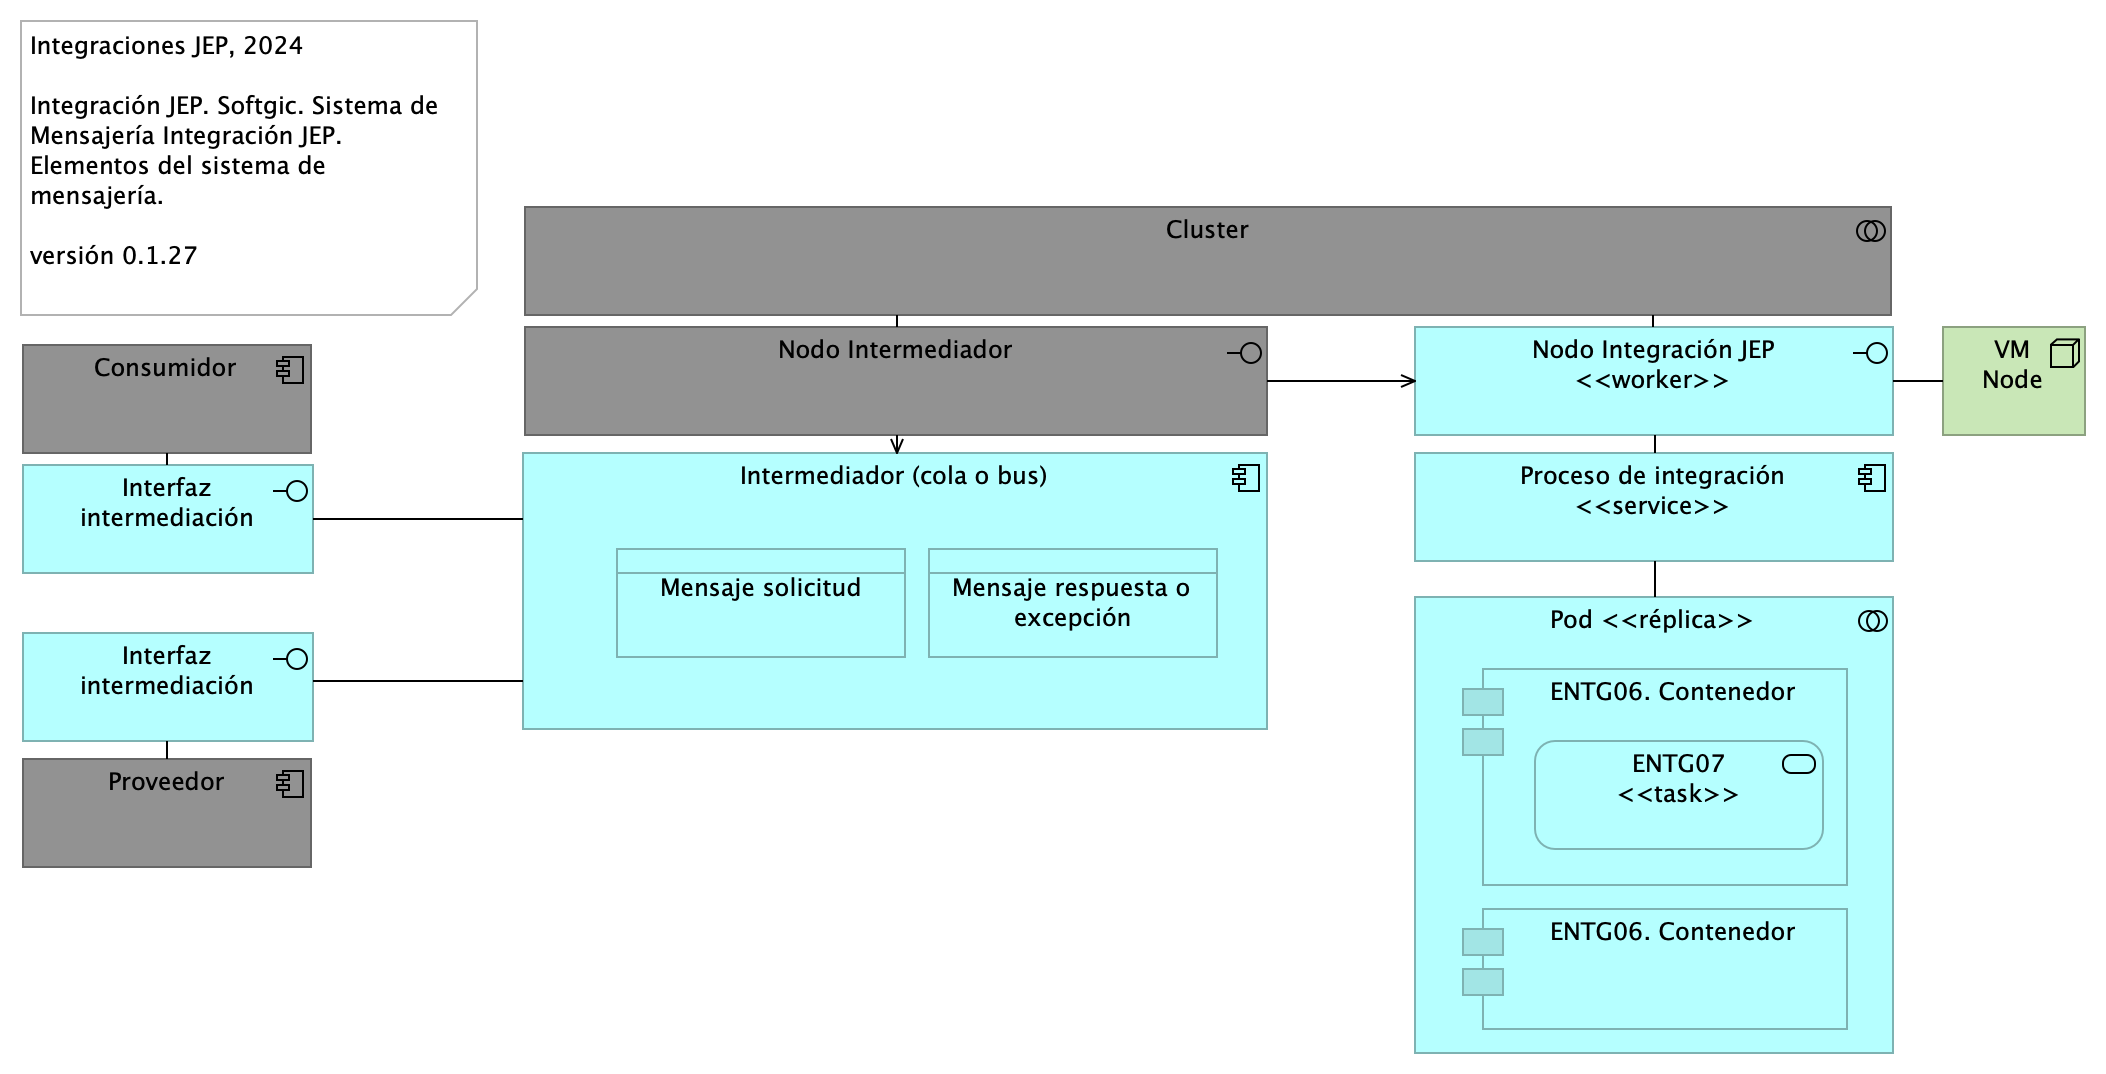
\includegraphics[width=\textwidth,height=5.20833in]{images/04.ING.3n.3.SistemadeMensajeríaIntegraciónJEP.png}
\caption{04.ING.3n.3. Sistema de Mensajería Integración JEP.
\emph{Fuente: Repositorio arquitectura Integración JEP
(2024)}}\label{fig:id-402ea0d886a14c76a3459332f1f2953c}
\end{figure}

\subsubsection{Catálogo de
Elementos}\label{sec:catuxe1logo-de-elementos-5}

\begin{longtable}[]{@{}
  >{\raggedright\arraybackslash}p{(\columnwidth - 4\tabcolsep) * \real{0.3000}}
  >{\raggedright\arraybackslash}p{(\columnwidth - 4\tabcolsep) * \real{0.2000}}
  >{\raggedright\arraybackslash}p{(\columnwidth - 4\tabcolsep) * \real{0.5000}}@{}}
\toprule\noalign{}
\begin{minipage}[b]{\linewidth}\raggedright
Nombre
\end{minipage} & \begin{minipage}[b]{\linewidth}\raggedright
Tipo
\end{minipage} & \begin{minipage}[b]{\linewidth}\raggedright
Documentación
\end{minipage} \\
\midrule\noalign{}
\endhead
\bottomrule\noalign{}
\endlastfoot
Cluster & Application Collaboration & Orquestador de nodos y servicios
(contendores) de la JEP. \\
& & \\
Consumidor & Application Component & Aplicación o servicio consumidor.
Emite mensajes de petición al proveedor de datos o comandos. \\
& & \\
ENTG06. Contenedor & Application Component & Contenedores de los
servicios de integración del proyecto desplegados en la infraestructura
tecnológica JEP. \\
& & \\
ENTG07 (task) & Application Service & Servicios de integración del
proyecto desplegados en la infraestructura tecnológica JEP. \\
& & \\
Interfaz intermediación & Application Interface & API de transporte de
mensajjes. Protocolo JMS, XMQ, MSMQ, etc. \\
& & \\
Intermediador (cola o bus) & Application Component & Bus de Red Hat,
aplicación cliente Quarkus, o intermediador de integración Apache
Camel. \\
Mensaje respuesta o excepción & Data Object & Formato predefinido de
intercambio de datos. \\
Mensaje solicitud & Data Object & Formato predefinido de intercambio de
datos. \\
Nodo Integración JEP (worker) & Application Collaboration & Nodo lógico
en donde corren los contenedores. \\
& & \\
Nodo Intermediador & Application Interface & Nodo lógico en donde corren
los contenedores. \\
& & \\
Proceso de integración (kb service) & Application Interface & Definición
de un proceso de trabajo de integración desplegable. \\
\end{longtable}

\textbar{} \textbar{} Proveedor \textbar{} Application Component
\textbar{} Aplicación o servicio proveedor. Emite mensajes de respuesta
al consumidor de datos o comandos. \textbar{} \textbar{} VM Node
\textbar{} Node \textbar{} Nodo físico donde corren los procesos del
sistema operativo. \textbar{}

Table: Elementos de la vista.
\{\#tbl:tblelement-04.ING.3n.3.SistemadeMensajeríaIntegraciónJEP-id\}

\newpage

\section{Modelo de Requerimientos de Interoperabilidad Proyecto
JEP}\label{sec:modelo-de-requerimientos-de-interoperabilidad-proyecto-jep}

\subsection{Requerimientos de Integración
JEP}\label{sec:requerimientos-de-integraciuxf3n-jep}

\begin{quote}
Modelo de Requerimientos Proyecto Integración JEP, 2024. Softgic.
Requerimientos, condiciones técnicas, solución del proyecto Integración
JEP, 2024. Versión 0.1.43
\end{quote}

Documentación de requerimientos del proyecto de integración JEP, 2024.
Implementados mediante el modelo de producción del proyecto.

Para la implementación de los ítems relacionados en el Anexo Nro. 1.1 --
Anexo técnico evolución plataforma de interoperabilidad -- Ficha Técnica
la hoja ``Categorías de Cotización'' contiene las necesidades a
contratar en el ámbito de la evolución tecnológica del modelo de
interoperabilidad y los desarrollos de interoperabilidad tanto con
sistemas internos, como con entidades externas. En la hoja ``Estándares
Desarrollo y Producto'' del archivo mencionado se indican los estándares
recomendados por el fabricante, para tener en cuenta en la entrega de
los servicios que se cotizan.

El Anexo Nro. 1.2 -- Acuerdos de Niveles de Servicio, explica el
procedimiento con el que se dará atención a consultas o solución de
incidencias, tanto en los sistemas operativos, como en los servicios de
interoperabilidad existentes en la actualidad y aquellos que se
contratarán en este proceso, en el sistema Bus de Interoperabilidad
implementado en la Jurisdicción Especial para la Paz.

-- Documento: Justificativo de la Contratación Invitación Pública

\begin{figure}
\centering
\includegraphics[width=\textwidth,height=5.20833in]{images/05.REQR.1n.RequerimientosServiciosdeIntegración.png}
\caption{05.REQR.1n. Requerimientos Servicios de Integración.
\emph{Fuente: Repositorio arquitectura Integración JEP
(2024)}}\label{fig:id-062616daaa1d4d8990681b58bc54ce3d}
\end{figure}

\subsubsection{Catálogo de
Elementos}\label{sec:catuxe1logo-de-elementos-6}

\begin{longtable}[]{@{}
  >{\raggedright\arraybackslash}p{(\columnwidth - 4\tabcolsep) * \real{0.3000}}
  >{\raggedright\arraybackslash}p{(\columnwidth - 4\tabcolsep) * \real{0.2000}}
  >{\raggedright\arraybackslash}p{(\columnwidth - 4\tabcolsep) * \real{0.5000}}@{}}
\toprule\noalign{}
\begin{minipage}[b]{\linewidth}\raggedright
Nombre
\end{minipage} & \begin{minipage}[b]{\linewidth}\raggedright
Tipo
\end{minipage} & \begin{minipage}[b]{\linewidth}\raggedright
Documentación
\end{minipage} \\
\midrule\noalign{}
\endhead
\bottomrule\noalign{}
\endlastfoot
REQR11. Integración gestión médica & Requirement & Documentación del
requerimiento de integración de la gestión médica JEP. Exposición de las
capacidades Radicar MP y Indexar Imagen. \\
\end{longtable}

Fuente: gestionMedidaProteccion (pdf).

\subsubsection{Índice de la documentación (casos de
uso)}\label{sec:uxedndice-de-la-documentaciuxf3n-casos-de-uso}

\begin{enumerate}
\def\labelenumi{\arabic{enumi}.}
\tightlist
\item
  Caso de Uso 1. Integrar Radicar MP
\item
  Caso de Uso 2. Integrar Indexar Imagen
\end{enumerate}

\textbar{} \textbar{} API en contenedores \textbar{} Technology Service
\textbar{} 1. La solución de administración de API debe admitir la
instalación de API Gateways en contenedores tanto dentro de una
plataforma Kubernetes o utilizando en motor de contenedor aprobado por
la especificación OCI. \textbar{} \textbar{} Aplicación de políticas API
\textbar{} Technology Service \textbar{} 1. La herramienta API Gateway
debe controlar la ejecución de llamadas, recopilar métricas, aplicar
políticas y límites de ejecución; \textbar{} \textbar{} Apoyar la
gestión médica \textbar{} Value \textbar{} Valor: el requerimientos
genera entregables de valor para la gestión médica de JEP. \textbar{}
\textbar{} Comunicación Legali x Conti \textbar{} Value \textbar{}
Valor: el requerimientos genera entregables de valor para la integración
de aplicaciones de JEP. \textbar{} \textbar{} Comunicación Legali x
Protecti \textbar{} Value \textbar{} Valor: el requerimientos genera
entregables de valor para la integración de aplicaciones de JEP.
\textbar{} \textbar{} Contractual \textbar{} Goal \textbar{} Objetivo:
el requerimiento tiene carácter contractual. \textbar{} \textbar{}
Conversión de mensajes \textbar{} Technology Service \textbar{} 1. Debe
poder convertir mensajes a / desde: XML, objetos Java, JSON, REST, CSV.
\textbar{} \textbar{} Generar API \textbar{} Technology Service
\textbar{} 1. La solución debe implementar la publicación de
microservicios que generen múltiples API para plataformas y clientes
específicos con las funciones específicas y protocolos requeridos por
cada plataforma. \textbar{} \textbar{} Gestión de tokens de acceso
\textbar{} Technology Service \textbar{} 1. Debe ser posible gestionar
la creación de un token de acceso, eligiendo su alcance, permiso y otras
cualidades a nivel de autenticación. \textbar{} \textbar{} Levantamiento
\textbar{} Constraint \textbar{} Restricción: el requerimiento está
condicionado por la completitud del levantamiento. \textbar{} \textbar{}
Métricas con Prometheus \textbar{} Technology Service \textbar{} 1. La
solución debería exponer métricas con integración nativa al software
Prometheus. \textbar{} \textbar{} Múltiples protocols \textbar{}
Technology Service \textbar{} 1. La solución debe implementar el
habilitar la traducción de múltiples protocolos del consumidor a un
protocolo específico del microservicio ofrecido a través de un API
Gateway. \textbar{} \textbar{} No Funcional \textbar{} Goal \textbar{}
Condiciones técnicas que debe cumplir la solución de interoperabilidad
JEP. \textbar{} \textbar{} Observabilidad de API \textbar{} Technology
Service \textbar{} 1. Debe permitir ver las llamadas a la API y separar
los códigos de retorno HTTP. \textbar{} \textbar{} Plataforma Openshift
\textbar{} Technology Service \textbar{} 1. Los servicios se deberán
implementar bajo la plataforma Openshift de RedHat. \textbar{}
\textbar{} Prácticas de integración empresarial \textbar{} Technology
Service \textbar{} 1. La infraestructura debe distribuirse de modo que
las integraciones, construidas a partir de EIP (patrones de integración
empresarial) y conectores predefinidos, se implementen en la
infraestructura nativa del contenedor para adaptarse y escalar
rápidamente \textbar{} \textbar{} REQR12. Integración Legali x Protecti
\textbar{} Requirement \textbar{} Documentación API de integración.
Creación de documento técnico para el consumo de servicios web.

Fuente: Documentación técnica - API Integración - Consulta de personas
(pdf). Pedro Escobar, ing.

\subsubsection{Índice de la documentación (casos de
uso)}\label{sec:uxedndice-de-la-documentaciuxf3n-casos-de-uso-1}

\begin{enumerate}
\def\labelenumi{\arabic{enumi}.}
\tightlist
\item
  Personas
\item
  Persona
\item
  Dirección de la persona
\item
  Teléfono de la persona
\item
  Procesos de la persona
\item
  Detalles del proceso
\item
  Partes del proceso
\item
  Asociación de parte del proceso
\item
  Paginación
\end{enumerate}

\textbar{} \textbar{} REQR2. Condiciones tecnológicas JEP \textbar{}
Requirement \textbar{} 1. La solución debe implementar el habilitar la
traducción de múltiples protocolos del consumidor a un protocolo
específico del microservicio ofrecido a través de un API Gateway 1. La
solución debe implementar la publicación de microservicios que generen
múltiples API para plataformas y clientes específicos con las funciones
específicas y protocolos requeridos por cada plataforma 1. La solución
debe implementar un mecanismo de hacer la trazabilidad, uso y registro
de actividades de los microservicios. 1. Debe permitir la integración
con un servicio de directorio corporativo que puede servir como
administrador de identidad corporativa. Por lo tanto, la solución debe
poder actuar como Administrador de acceso (Identity Access Manager -
IaM) mientras que el Servicio de directorio sirve como Administrador e
Identidades (Identity Manager - IdM). 1. Debe admitir la transformación
y el enrutamiento hacia / desde SOAP / HTTP a los servicios REST. 1.
Debe poder convertir mensajes a / desde: XML, objetos Java, JSON, REST,
CSV. 1. Debe proporcionar componentes para la transformación utilizando
modelos predefinidos (plantillas). 1. La infraestructura debe
distribuirse de modo que las integraciones, construidas a partir de EIP
(patrones de integración empresarial) y conectores predefinidos, se
implementen en la infraestructura nativa del contenedor para adaptarse y
escalar rápidamente 1. La solución debería exponer métricas con
integración nativa al software Prometheus 1. Debe ser posible gestionar
la creación de un token de acceso, eligiendo su alcance, permiso y otras
cualidades a nivel de autenticación 1. La solución de administración de
API debe admitir la instalación de API Gateways en contenedores tanto
dentro de una plataforma Kubernetes o utilizando en motor de contenedor
aprobado por la especificación OCI 1. Debe permitir ver las llamadas a
la API y separar los códigos de retorno HTTP. 1. La herramienta API
Gateway debe controlar la ejecución de llamadas, recopilar métricas,
aplicar políticas y límites de ejecución; 1. Para permitir
interoperabilidad debe habilitar transporte de mensajes y conectarse
entre ellos. Los mecanismos de transporte deben incluir Java Messaging
Service (JMS), Active MQ y asi mismo protocolos de comunicación tal como
HTTP/HTTPS,SMTP, entre otros 1. Se debe contar con la característica de
Single Sign On (SSO) 1. Los servicios se deberán implementar bajo la
plataforma Openshift de RedHat 1. Se debe contemplar dentro de estos
desarrollos la Transferencia de archivos utilizando el esquema de
almacenamiento de Openshift ODF asociado a un esquema NFS,
Administración de Personas, Consulta y transferencia de expedientes o
partes de expedientes y anexos, etc

Fuente: Anexo Técnico 1.1 Pliego del Proyecto \textbar{} \textbar{}
REQR3. Integración con Sistema Conti x Plani \textbar{} Requirement
\textbar{} Atendiendo la necesidad de la Subdirección de Contratación de
implementar el flujo de gestión precontractual en el sistema de Gestión
Documental - Conti se requiere contar con la información de los ítems
del Plan Anual de Adquisiciones -- PAA para iniciar el proceso, la cual
se encuentra gestionada en el Sistema de Gestión y Planeación
Institucional PLANi.

\subsubsection{Índice de la documentación (casos de
uso)}\label{sec:uxedndice-de-la-documentaciuxf3n-casos-de-uso-2}

\begin{enumerate}
\def\labelenumi{\arabic{enumi}.}
\tightlist
\item
  Integración. Ingreso a Conti
\item
  Integración. Consulta ítem de Conti
\item
  Integración. Radicar ítem 1.Integración. Generación de documentos
\end{enumerate}

\textbar{} \textbar{} SINT1. Integración. Ingreso a Conti \textbar{}
Application Service \textbar{} Tareas de desarrollo

\begin{itemize}
\item
  Interoperabilidad IOP1. Transporte / Entrega Consulta Negocio
\item
  Modelo de datos (XML, RBDMS, \ldots)
\item
  Esquema de datos (XSD, DTD, JSON-E\ldots)
\item
  Contratos de interoperabilidad (WSDL, API\ldots)
\item
  Mensajes petición IN (API, XML\ldots)
\item
  Mensajes respuesta OUT (API, XML\ldots)
\item
  Mensajes excepción (API, XML\ldots)
\item
  Transporte (REST, SOAP)
\item
  Función lógica (JEE, \ldots)
\item
  Registro y envío de actividad \textbar{} \textbar{} SINT10. Integrar
  Radicar MP \textbar{} Application Service \textbar{} Tareas de
  desarrollo
\item
  Interoperabilidad IOP1. Transporte / Entrega Consulta Negocio
\item
  Modelo de datos (XML, RBDMS, \ldots)
\item
  Esquema de datos (XSD, DTD, JSON-E\ldots)
\item
  Contratos de interoperabilidad (WSDL, API\ldots)
\item
  Mensajes petición IN (API, XML\ldots)
\item
  Mensajes respuesta OUT (API, XML\ldots)
\item
  Mensajes excepción (API, XML\ldots)
\item
  Transporte (REST, SOAP)
\item
  Función lógica (JEE, \ldots)
\item
  Registro y envío de actividad \textbar{} \textbar{} SINT11. Integrar
  Indexar Imagen \textbar{} Application Service \textbar{} Tareas de
  desarrollo
\item
  Interoperabilidad IOP1. Transporte / Entrega Consulta Negocio
\item
  Modelo de datos (XML, RBDMS, \ldots)
\item
  Esquema de datos (XSD, DTD, JSON-E\ldots)
\item
  Contratos de interoperabilidad (WSDL, API\ldots)
\item
  Mensajes petición IN (API, XML\ldots)
\item
  Mensajes respuesta OUT (API, XML\ldots)
\item
  Mensajes excepción (API, XML\ldots)
\item
  Transporte (REST, SOAP)
\item
  Función lógica (JEE, \ldots)
\item
  Registro y envío de actividad \textbar{} \textbar{} SINT2.
  Integración. Consulta ítem de Conti \textbar{} Application Service
  \textbar{} Tareas de desarrollo
\item
  Interoperabilidad IOP1. Transporte / Entrega Consulta Negocio
\item
  Modelo de datos (XML, RBDMS, \ldots)
\item
  Esquema de datos (XSD, DTD, JSON-E\ldots)
\item
  Contratos de interoperabilidad (WSDL, API\ldots)
\item
  Mensajes petición IN (API, XML\ldots)
\item
  Mensajes respuesta OUT (API, XML\ldots)
\item
  Mensajes excepción (API, XML\ldots)
\item
  Transporte (REST, SOAP)
\item
  Función lógica (JEE, \ldots)
\item
  Registro y envío de actividad \textbar{} \textbar{} SINT20. Personas
  \textbar{} Application Service \textbar{} Tareas de desarrollo
\item
  Interoperabilidad IOP1. Transporte / Entrega Consulta Negocio\\
\item
  Modelo de datos (XML, RBDMS, \ldots)
\item
  Esquema de datos (XSD, DTD, JSON-E\ldots)
\item
  Contratos de interoperabilidad (WSDL, API\ldots)
\item
  Mensajes petición IN (API, XML\ldots)
\item
  Mensajes respuesta OUT (API, XML\ldots)
\item
  Mensajes excepción (API, XML\ldots)
\item
  Transporte (REST, SOAP)
\item
  Función lógica (JEE, \ldots)
\item
  Registro y envío de actividad \textbar{} \textbar{} SINT21. Persona
  \textbar{} Application Service \textbar{} Tareas de desarrollo
\item
  Interoperabilidad IOP1. Transporte / Entrega Consulta Negocio\\
\item
  Modelo de datos (XML, RBDMS, \ldots)
\item
  Esquema de datos (XSD, DTD, JSON-E\ldots)
\item
  Contratos de interoperabilidad (WSDL, API\ldots)
\item
  Mensajes petición IN (API, XML\ldots)
\item
  Mensajes respuesta OUT (API, XML\ldots)
\item
  Mensajes excepción (API, XML\ldots)
\item
  Transporte (REST, SOAP)
\item
  Función lógica (JEE, \ldots)
\item
  Registro y envío de actividad \textbar{} \textbar{} SINT22. Dirección
  de la persona \textbar{} Application Service \textbar{} Tareas de
  desarrollo
\item
  Interoperabilidad IOP1. Transporte / Entrega Consulta Negocio\\
\item
  Modelo de datos (XML, RBDMS, \ldots)
\item
  Esquema de datos (XSD, DTD, JSON-E\ldots)
\item
  Contratos de interoperabilidad (WSDL, API\ldots)
\item
  Mensajes petición IN (API, XML\ldots)
\item
  Mensajes respuesta OUT (API, XML\ldots)
\item
  Mensajes excepción (API, XML\ldots)
\item
  Transporte (REST, SOAP)
\item
  Función lógica (JEE, \ldots)
\item
  Registro y envío de actividad \textbar{} \textbar{} SINT23. Partes del
  proceso \textbar{} Application Service \textbar{} Tareas de desarrollo
\item
  Interoperabilidad IOP1. Transporte / Entrega Consulta Negocio\\
\item
  Modelo de datos (XML, RBDMS, \ldots)
\item
  Esquema de datos (XSD, DTD, JSON-E\ldots)
\item
  Contratos de interoperabilidad (WSDL, API\ldots)
\item
  Mensajes petición IN (API, XML\ldots)
\item
  Mensajes respuesta OUT (API, XML\ldots)
\item
  Mensajes excepción (API, XML\ldots)
\item
  Transporte (REST, SOAP)
\item
  Función lógica (JEE, \ldots)
\item
  Registro y envío de actividad \textbar{} \textbar{} SINT23. Teléfono
  de la persona \textbar{} Application Service \textbar{} Tareas de
  desarrollo
\item
  Interoperabilidad IOP1. Transporte / Entrega Consulta Negocio\\
\item
  Modelo de datos (XML, RBDMS, \ldots)
\item
  Esquema de datos (XSD, DTD, JSON-E\ldots)
\item
  Contratos de interoperabilidad (WSDL, API\ldots)
\item
  Mensajes petición IN (API, XML\ldots)
\item
  Mensajes respuesta OUT (API, XML\ldots)
\item
  Mensajes excepción (API, XML\ldots)
\item
  Transporte (REST, SOAP)
\item
  Función lógica (JEE, \ldots)
\item
  Registro y envío de actividad \textbar{} \textbar{} SINT25. Procesos
  de la persona \textbar{} Application Service \textbar{} Tareas de
  desarrollo
\item
  Interoperabilidad IOP1. Transporte / Entrega Consulta Negocio\\
\item
  Modelo de datos (XML, RBDMS, \ldots)
\item
  Esquema de datos (XSD, DTD, JSON-E\ldots)
\item
  Contratos de interoperabilidad (WSDL, API\ldots)
\item
  Mensajes petición IN (API, XML\ldots)
\item
  Mensajes respuesta OUT (API, XML\ldots)
\item
  Mensajes excepción (API, XML\ldots)
\item
  Transporte (REST, SOAP)
\item
  Función lógica (JEE, \ldots)
\item
  Registro y envío de actividad \textbar{} \textbar{} SINT26. Asociación
  de parte del proceso \textbar{} Application Service \textbar{} Tareas
  de desarrollo
\item
  Interoperabilidad IOP1. Transporte / Entrega Consulta Negocio\\
\item
  Modelo de datos (XML, RBDMS, \ldots)
\item
  Esquema de datos (XSD, DTD, JSON-E\ldots)
\item
  Contratos de interoperabilidad (WSDL, API\ldots)
\item
  Mensajes petición IN (API, XML\ldots)
\item
  Mensajes respuesta OUT (API, XML\ldots)
\item
  Mensajes excepción (API, XML\ldots)
\item
  Transporte (REST, SOAP)
\item
  Función lógica (JEE, \ldots)
\item
  Registro y envío de actividad \textbar{} \textbar{} SINT26. Detalles
  del proceso \textbar{} Application Service \textbar{} Tareas de
  desarrollo
\item
  Interoperabilidad IOP1. Transporte / Entrega Consulta Negocio\\
\item
  Modelo de datos (XML, RBDMS, \ldots)
\item
  Esquema de datos (XSD, DTD, JSON-E\ldots)
\item
  Contratos de interoperabilidad (WSDL, API\ldots)
\item
  Mensajes petición IN (API, XML\ldots)
\item
  Mensajes respuesta OUT (API, XML\ldots)
\item
  Mensajes excepción (API, XML\ldots)
\item
  Transporte (REST, SOAP)
\item
  Función lógica (JEE, \ldots)
\item
  Registro y envío de actividad \textbar{} \textbar{} SINT27. Paginación
  \textbar{} Application Service \textbar{} Tareas de desarrollo
\item
  Interoperabilidad IOP1. Transporte / Entrega Consulta Negocio\\
\item
  Modelo de datos (XML, RBDMS, \ldots)
\item
  Esquema de datos (XSD, DTD, JSON-E\ldots)
\item
  Contratos de interoperabilidad (WSDL, API\ldots)
\item
  Mensajes petición IN (API, XML\ldots)
\item
  Mensajes respuesta OUT (API, XML\ldots)
\item
  Mensajes excepción (API, XML\ldots)
\item
  Transporte (REST, SOAP)
\item
  Función lógica (JEE, \ldots)
\item
  Registro y envío de actividad \textbar{} \textbar{} SINT3.
  Integración. Radicar ítem \textbar{} Application Service \textbar{}
  Tareas de desarrollo
\item
  Interoperabilidad IOP1. Transporte / Entrega Consulta Negocio
\item
  Modelo de datos (XML, RBDMS, \ldots)
\item
  Esquema de datos (XSD, DTD, JSON-E\ldots)
\item
  Contratos de interoperabilidad (WSDL, API\ldots)
\item
  Mensajes petición IN (API, XML\ldots)
\item
  Mensajes respuesta OUT (API, XML\ldots)
\item
  Mensajes excepción (API, XML\ldots)
\item
  Transporte (REST, SOAP)
\item
  Función lógica (JEE, \ldots)
\item
  Registro y envío de actividad \textbar{} \textbar{} SINT4.
  Integración. Generación de documentos \textbar{} Application Service
  \textbar{} Tareas de desarrollo
\item
  Interoperabilidad IOP1. Transporte / Entrega Consulta Negocio
\item
  Modelo de datos (XML, RBDMS, \ldots)
\item
  Esquema de datos (XSD, DTD, JSON-E\ldots)
\item
  Contratos de interoperabilidad (WSDL, API\ldots)
\item
  Mensajes petición IN (API, XML\ldots)
\item
  Mensajes respuesta OUT (API, XML\ldots)
\item
  Mensajes excepción (API, XML\ldots)
\item
  Transporte (REST, SOAP)
\item
  Función lógica (JEE, \ldots)
\item
  Registro y envío de actividad \textbar{} \textbar{} Single Sign On
  (SSO) \textbar{} Technology Service \textbar{} 1. Se debe contar con
  la característica de Single Sign On (SSO). \textbar{} \textbar{}
  Sistema de mensajes \textbar{} Technology Service \textbar{} 1. Para
  permitir interoperabilidad debe habilitar transporte de mensajes y
  conectarse entre ellos. Los mecanismos de transporte deben incluir
  Java Messaging Service (JMS), Active MQ y asi mismo protocolos de
  comunicación tal como HTTP/HTTPS, SMTP, entre otros. \textbar{}
  \textbar{} Transferencia de archivos \textbar{} Technology Service
  \textbar{} 1. Se debe contemplar dentro de estos desarrollos la
  transferencia de archivos utilizando el esquema de almacenamiento de
  Openshift ODF asociado a un esquema NFS, Administración de Personas,
  Consulta y transferencia de expedientes o partes de expedientes y
  anexos, etc . \textbar{} \textbar{} Transformación \textbar{}
  Technology Service \textbar{} 1. Debe proporcionar componentes para la
  transformación utilizando modelos predefinidos (plantillas).
  \textbar{} \textbar{} Transformación y enrutamiento \textbar{}
  Technology Service \textbar{} 1. Debe admitir la transformación y el
  enrutamiento hacia / desde SOAP / HTTP a los servicios REST.
  \textbar{} \textbar{} Trazabilidad \textbar{} Technology Service
  \textbar{} 1. La solución debe implementar un mecanismo de hacer la
  trazabilidad, uso y registro de actividades de los microservicios.
  \textbar{}
\end{itemize}

Table: Elementos de la vista.
\{\#tbl:tblelement-05.REQR.1n.RequerimientosServiciosdeIntegración-id\}

\newpage

\section{Modelo de Entrega y Despliegue de
Requerimientos}\label{sec:modelo-de-entrega-y-despliegue-de-requerimientos}

\subsection{Gestión de Entregas del
Requerimiento}\label{sec:gestiuxf3n-de-entregas-del-requerimiento}

\begin{quote}
Integraciones JEP, 2024 Integración JEP. Softgic. Plan de Entregas del
proyecto de integración JEP, iteraciones y Entregables por versión.
versión 0.1.4
\end{quote}

Documento de requerimientos, primera versión de entregas del proyecto
Integraciones JEP, 2024.

El requerimiento Integración con Sistema Conti x Plani (REQR3, en la
imagen) será entregado con la primera versión que se libere de la
solución de integración, actualmente en desarrollo por Softgic.

Este requerimiento REQR3 consta de dos iteraciones (Iteración 1 y 2, en
la imagen), las cuales a su vez, realizarán dos historias de integración
cada una (HU01, HU02, HU03, HU04, respectivamente).

Una vez concluidas la ejecución de las dos iteraciones, y sus historias
de integración contenidas, realizaremos la entrega de los 4 primeros
servicios de integración desplegables en el namespace de Openshift de
desarrollo de la JEP.

\begin{figure}
\centering
\includegraphics[width=\textwidth,height=5.20833in]{images/06.ENTRG.1n.1a.GestiónEntregasdeRequerimientos.png}
\caption{06.ENTRG.1n.1a. Gestión Entregas de Requerimientos.
\emph{Fuente: Repositorio arquitectura Integración JEP
(2024)}}\label{fig:id-c31668d4d5dd44309f42fdd5fb2a7a53}
\end{figure}

\subsubsection{Catálogo de
Elementos}\label{sec:catuxe1logo-de-elementos-7}

\begin{longtable}[]{@{}
  >{\raggedright\arraybackslash}p{(\columnwidth - 4\tabcolsep) * \real{0.3000}}
  >{\raggedright\arraybackslash}p{(\columnwidth - 4\tabcolsep) * \real{0.2000}}
  >{\raggedright\arraybackslash}p{(\columnwidth - 4\tabcolsep) * \real{0.5000}}@{}}
\toprule\noalign{}
\begin{minipage}[b]{\linewidth}\raggedright
Nombre
\end{minipage} & \begin{minipage}[b]{\linewidth}\raggedright
Tipo
\end{minipage} & \begin{minipage}[b]{\linewidth}\raggedright
Documentación
\end{minipage} \\
\midrule\noalign{}
\endhead
\bottomrule\noalign{}
\endlastfoot
Integración Conti & Deliverable & Épica de entrega de la solución de
integración JEP, 2024, que contiene las iteraciones que realizarán la
característica `Integrar operaciones Conti'. \\
\end{longtable}

\textbar{} \textbar{} Integrar operaciones Conti \textbar{} Driver
\textbar{} Característica de integración de Conti contenido en la
solución de integración JEP, 2024. \textbar{} \textbar{} REQR3.
Integración con Sistema Conti x Plani \textbar{} Requirement \textbar{}
Atendiendo la necesidad de la Subdirección de Contratación de
implementar el flujo de gestión precontractual en el sistema de Gestión
Documental - Conti se requiere contar con la información de los ítems
del Plan Anual de Adquisiciones -- PAA para iniciar el proceso, la cual
se encuentra gestionada en el Sistema de Gestión y Planeación
Institucional PLANi.

\subsubsection{Índice de la documentación (casos de
uso)}\label{sec:uxedndice-de-la-documentaciuxf3n-casos-de-uso-3}

\begin{enumerate}
\def\labelenumi{\arabic{enumi}.}
\tightlist
\item
  Integración. Ingreso a Conti
\item
  Integración. Consulta ítem de Conti
\item
  Integración. Radicar ítem 1.Integración. Generación de documentos
\end{enumerate}

\textbar{} \textbar{} SINT1. Integración. Ingreso a Conti \textbar{}
Application Service \textbar{} Tareas de desarrollo

\begin{itemize}
\item
  Interoperabilidad IOP1. Transporte / Entrega Consulta Negocio
\item
  Modelo de datos (XML, RBDMS, \ldots)
\item
  Esquema de datos (XSD, DTD, JSON-E\ldots)
\item
  Contratos de interoperabilidad (WSDL, API\ldots)
\item
  Mensajes petición IN (API, XML\ldots)
\item
  Mensajes respuesta OUT (API, XML\ldots)
\item
  Mensajes excepción (API, XML\ldots)
\item
  Transporte (REST, SOAP)
\item
  Función lógica (JEE, \ldots)
\item
  Registro y envío de actividad \textbar{} \textbar{} SINT2.
  Integración. Consulta ítem de Conti \textbar{} Application Service
  \textbar{} Tareas de desarrollo
\item
  Interoperabilidad IOP1. Transporte / Entrega Consulta Negocio
\item
  Modelo de datos (XML, RBDMS, \ldots)
\item
  Esquema de datos (XSD, DTD, JSON-E\ldots)
\item
  Contratos de interoperabilidad (WSDL, API\ldots)
\item
  Mensajes petición IN (API, XML\ldots)
\item
  Mensajes respuesta OUT (API, XML\ldots)
\item
  Mensajes excepción (API, XML\ldots)
\item
  Transporte (REST, SOAP)
\item
  Función lógica (JEE, \ldots)
\item
  Registro y envío de actividad \textbar{} \textbar{} SINT3.
  Integración. Radicar ítem \textbar{} Application Service \textbar{}
  Tareas de desarrollo
\item
  Interoperabilidad IOP1. Transporte / Entrega Consulta Negocio
\item
  Modelo de datos (XML, RBDMS, \ldots)
\item
  Esquema de datos (XSD, DTD, JSON-E\ldots)
\item
  Contratos de interoperabilidad (WSDL, API\ldots)
\item
  Mensajes petición IN (API, XML\ldots)
\item
  Mensajes respuesta OUT (API, XML\ldots)
\item
  Mensajes excepción (API, XML\ldots)
\item
  Transporte (REST, SOAP)
\item
  Función lógica (JEE, \ldots)
\item
  Registro y envío de actividad \textbar{} \textbar{} SINT4.
  Integración. Generación de documentos \textbar{} Application Service
  \textbar{} Tareas de desarrollo
\item
  Interoperabilidad IOP1. Transporte / Entrega Consulta Negocio
\item
  Modelo de datos (XML, RBDMS, \ldots)
\item
  Esquema de datos (XSD, DTD, JSON-E\ldots)
\item
  Contratos de interoperabilidad (WSDL, API\ldots)
\item
  Mensajes petición IN (API, XML\ldots)
\item
  Mensajes respuesta OUT (API, XML\ldots)
\item
  Mensajes excepción (API, XML\ldots)
\item
  Transporte (REST, SOAP)
\item
  Función lógica (JEE, \ldots)
\item
  Registro y envío de actividad \textbar{}
\end{itemize}

Table: Elementos de la vista.
\{\#tbl:tblelement-06.ENTRG.1n.1a.GestiónEntregasdeRequerimientos-id\}

\subsection{Despliegue de Entregas de
Requerimientos}\label{sec:despliegue-de-entregas-de-requerimientos}

\begin{quote}
Integraciones JEP, 2024 Integración JEP. Softgic. Plan de Entregas del
proyecto de integración y despliegue JEP, iteraciones y Entregables por
versión. versión 0.1.14
\end{quote}

Los servicios implementados contenidos en los requerimientos se pueden
desplegar sobre la red de unidades de despliegue (pods) dispuesta por la
JEP y acordada con el contratista.

En esta organización propuesta, los servicios de integración
implementados pueden ser desplegados en uno, o varios contenedores, y en
unidades de despliegue (pods) distintas.

\begin{figure}
\centering
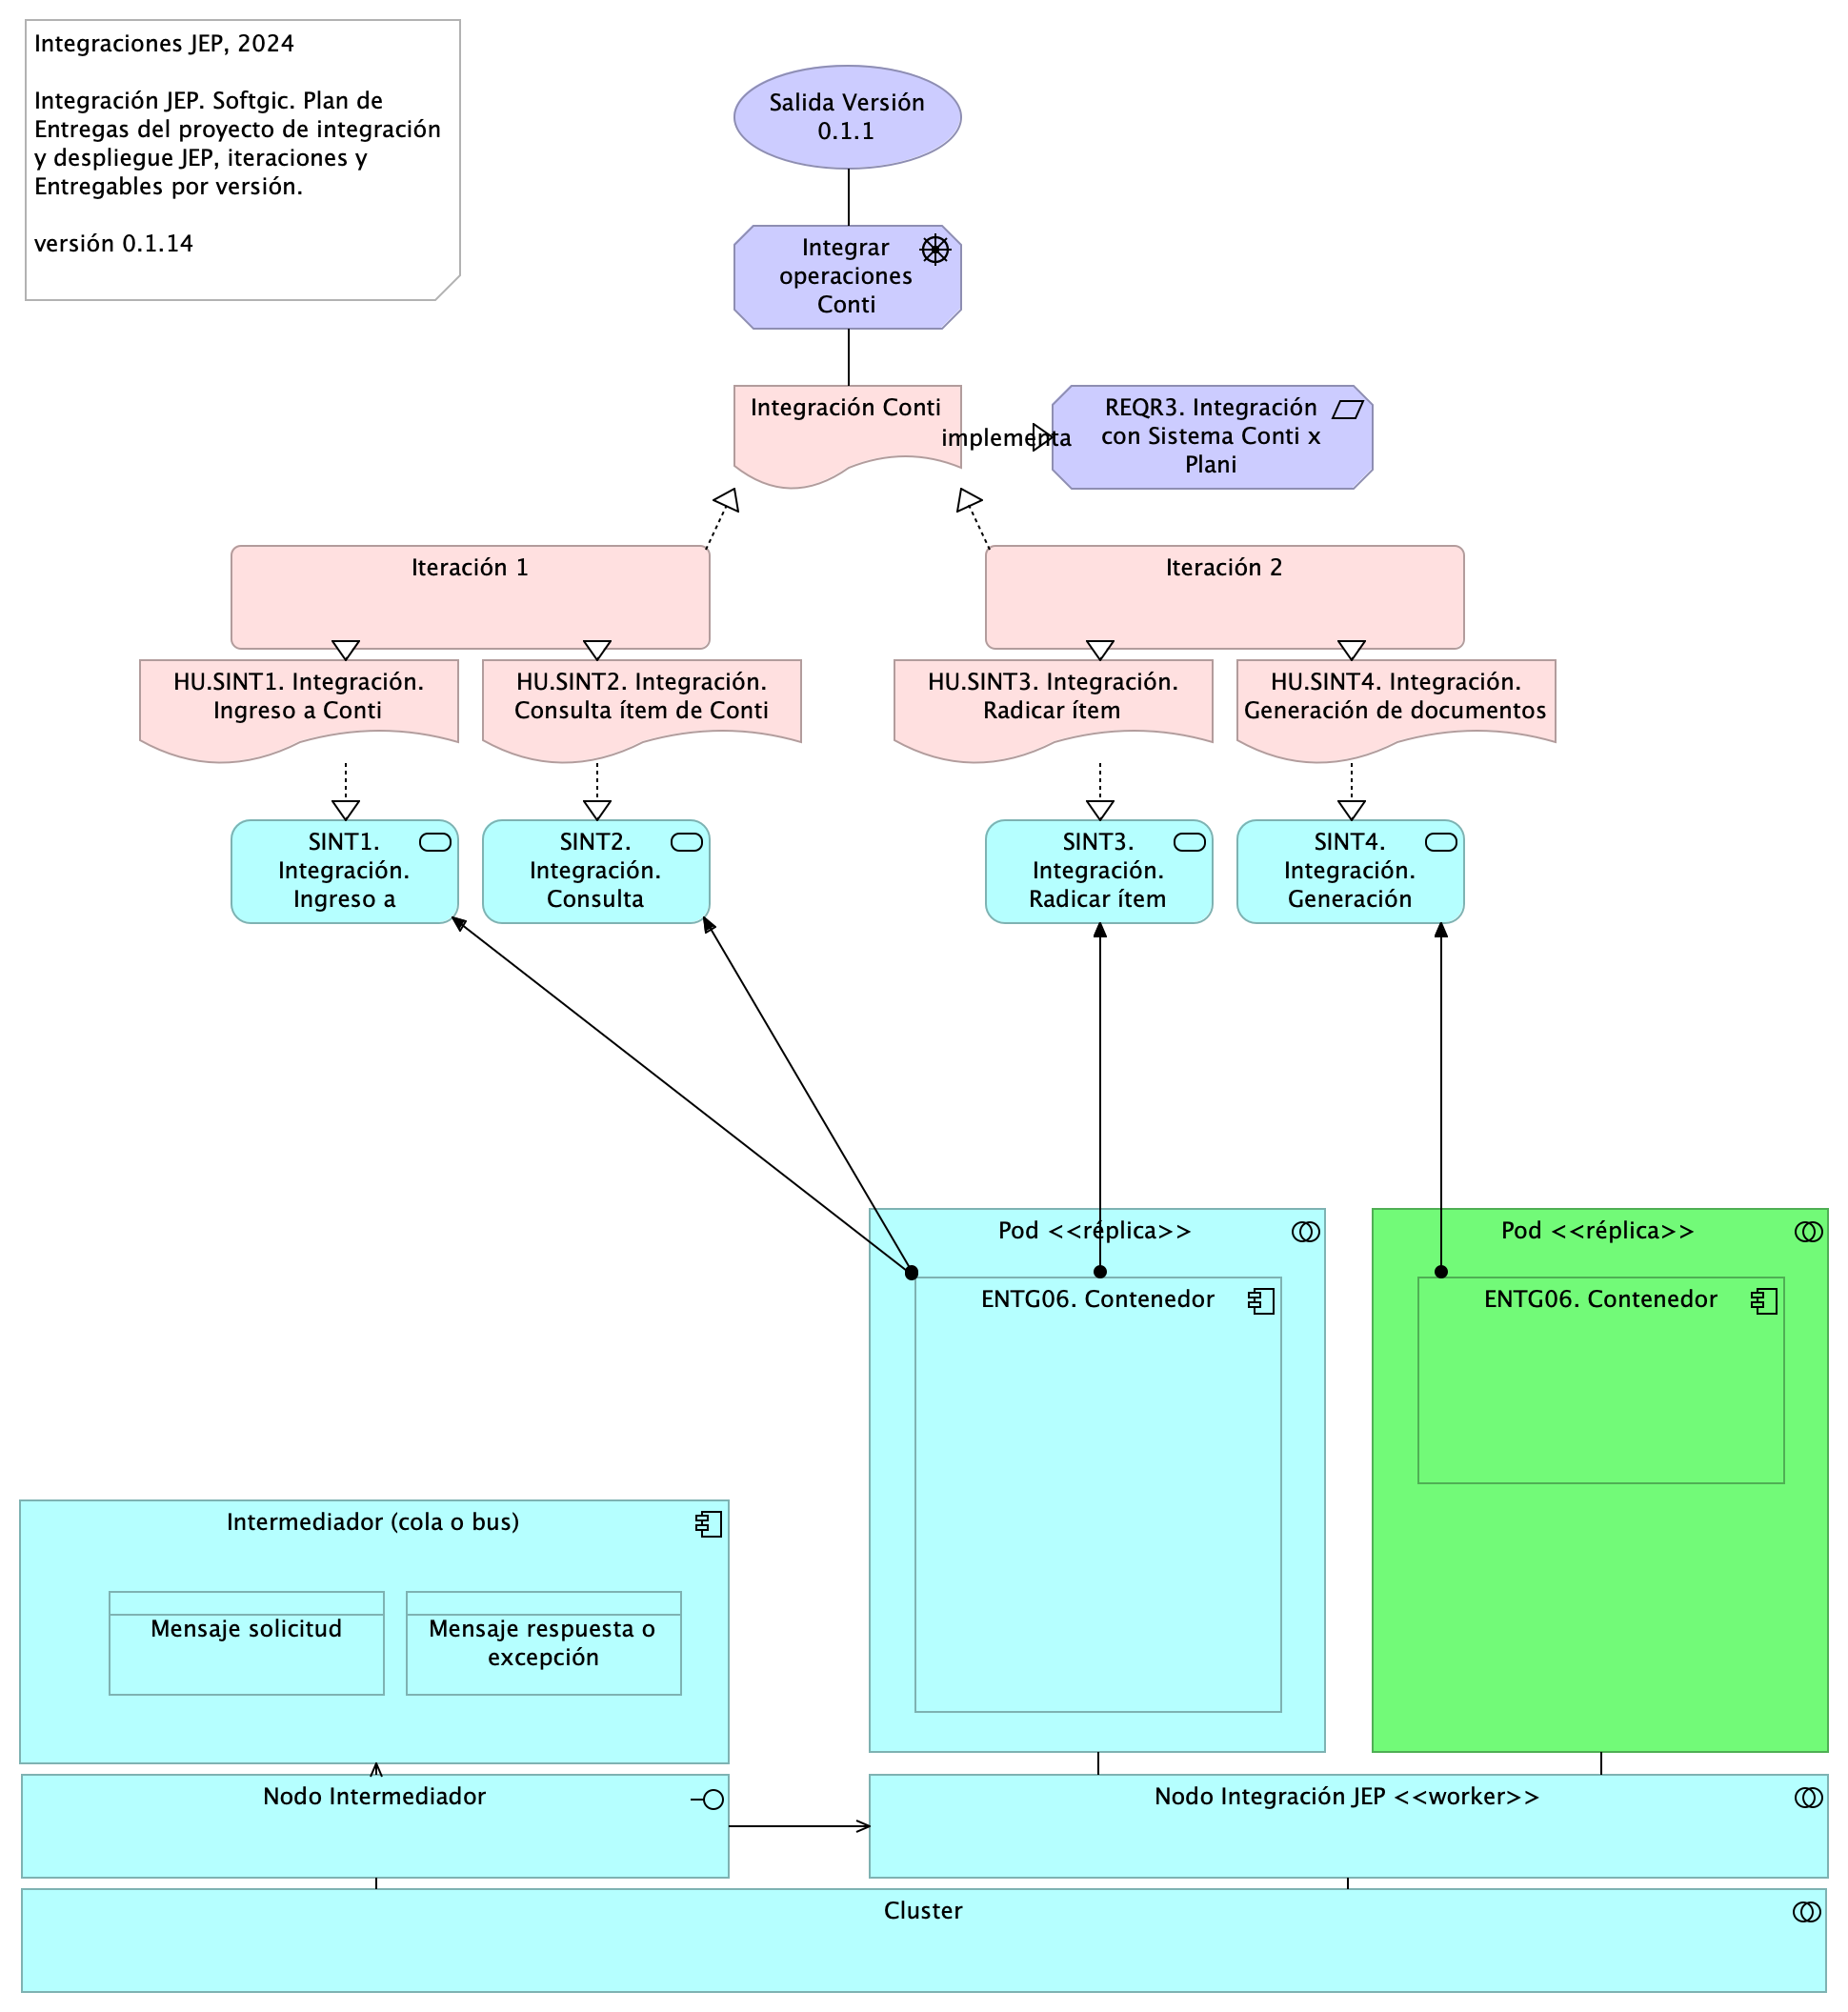
\includegraphics[width=\textwidth,height=5.20833in]{images/06.ENTRG.1n.1a.1.DespliegueEntregasdeRequerimiento.png}
\caption{06.ENTRG.1n.1a.1. Despliegue Entregas de Requerimiento.
\emph{Fuente: Repositorio arquitectura Integración JEP
(2024)}}\label{fig:id-203e737545e449e59334b47d3034d956}
\end{figure}

\subsubsection{Catálogo de
Elementos}\label{sec:catuxe1logo-de-elementos-8}

\begin{longtable}[]{@{}
  >{\raggedright\arraybackslash}p{(\columnwidth - 4\tabcolsep) * \real{0.3000}}
  >{\raggedright\arraybackslash}p{(\columnwidth - 4\tabcolsep) * \real{0.2000}}
  >{\raggedright\arraybackslash}p{(\columnwidth - 4\tabcolsep) * \real{0.5000}}@{}}
\toprule\noalign{}
\begin{minipage}[b]{\linewidth}\raggedright
Nombre
\end{minipage} & \begin{minipage}[b]{\linewidth}\raggedright
Tipo
\end{minipage} & \begin{minipage}[b]{\linewidth}\raggedright
Documentación
\end{minipage} \\
\midrule\noalign{}
\endhead
\bottomrule\noalign{}
\endlastfoot
Cluster & Application Collaboration & Orquestador de nodos y servicios
(contendores) de la JEP. \\
& & \\
ENTG06. Contenedor & Application Component & Contenedores de los
servicios de integración del proyecto desplegados en la infraestructura
tecnológica JEP. \\
& & \\
Integración Conti & Deliverable & Épica de entrega de la solución de
integración JEP, 2024, que contiene las iteraciones que realizarán la
característica `Integrar operaciones Conti'. \\
\end{longtable}

\textbar{} \textbar{} Integrar operaciones Conti \textbar{} Driver
\textbar{} Característica de integración de Conti contenido en la
solución de integración JEP, 2024. \textbar{} \textbar{} Intermediador
(cola o bus) \textbar{} Application Component \textbar{} Bus de Red Hat,
aplicación cliente Quarkus, o intermediador de integración Apache Camel.
\textbar{} \textbar{} Mensaje respuesta o excepción \textbar{} Data
Object \textbar{} Formato predefinido de intercambio de datos.
\textbar{} \textbar{} Mensaje solicitud \textbar{} Data Object
\textbar{} Formato predefinido de intercambio de datos. \textbar{}
\textbar{} Nodo Integración JEP (worker) \textbar{} Application
Collaboration \textbar{} Nodo lógico en donde corren los contenedores.
\textbar{} \textbar{} Nodo Intermediador \textbar{} Application
Interface \textbar{} Nodo lógico en donde corren los contenedores.
\textbar{} \textbar{} REQR3. Integración con Sistema Conti x Plani
\textbar{} Requirement \textbar{} Atendiendo la necesidad de la
Subdirección de Contratación de implementar el flujo de gestión
precontractual en el sistema de Gestión Documental - Conti se requiere
contar con la información de los ítems del Plan Anual de Adquisiciones
-- PAA para iniciar el proceso, la cual se encuentra gestionada en el
Sistema de Gestión y Planeación Institucional PLANi.

\subsubsection{Índice de la documentación (casos de
uso)}\label{sec:uxedndice-de-la-documentaciuxf3n-casos-de-uso-4}

\begin{enumerate}
\def\labelenumi{\arabic{enumi}.}
\tightlist
\item
  Integración. Ingreso a Conti
\item
  Integración. Consulta ítem de Conti
\item
  Integración. Radicar ítem 1.Integración. Generación de documentos
\end{enumerate}

\textbar{} \textbar{} SINT1. Integración. Ingreso a Conti \textbar{}
Application Service \textbar{} Tareas de desarrollo

\begin{itemize}
\item
  Interoperabilidad IOP1. Transporte / Entrega Consulta Negocio
\item
  Modelo de datos (XML, RBDMS, \ldots)
\item
  Esquema de datos (XSD, DTD, JSON-E\ldots)
\item
  Contratos de interoperabilidad (WSDL, API\ldots)
\item
  Mensajes petición IN (API, XML\ldots)
\item
  Mensajes respuesta OUT (API, XML\ldots)
\item
  Mensajes excepción (API, XML\ldots)
\item
  Transporte (REST, SOAP)
\item
  Función lógica (JEE, \ldots)
\item
  Registro y envío de actividad \textbar{} \textbar{} SINT2.
  Integración. Consulta ítem de Conti \textbar{} Application Service
  \textbar{} Tareas de desarrollo
\item
  Interoperabilidad IOP1. Transporte / Entrega Consulta Negocio
\item
  Modelo de datos (XML, RBDMS, \ldots)
\item
  Esquema de datos (XSD, DTD, JSON-E\ldots)
\item
  Contratos de interoperabilidad (WSDL, API\ldots)
\item
  Mensajes petición IN (API, XML\ldots)
\item
  Mensajes respuesta OUT (API, XML\ldots)
\item
  Mensajes excepción (API, XML\ldots)
\item
  Transporte (REST, SOAP)
\item
  Función lógica (JEE, \ldots)
\item
  Registro y envío de actividad \textbar{} \textbar{} SINT3.
  Integración. Radicar ítem \textbar{} Application Service \textbar{}
  Tareas de desarrollo
\item
  Interoperabilidad IOP1. Transporte / Entrega Consulta Negocio
\item
  Modelo de datos (XML, RBDMS, \ldots)
\item
  Esquema de datos (XSD, DTD, JSON-E\ldots)
\item
  Contratos de interoperabilidad (WSDL, API\ldots)
\item
  Mensajes petición IN (API, XML\ldots)
\item
  Mensajes respuesta OUT (API, XML\ldots)
\item
  Mensajes excepción (API, XML\ldots)
\item
  Transporte (REST, SOAP)
\item
  Función lógica (JEE, \ldots)
\item
  Registro y envío de actividad \textbar{} \textbar{} SINT4.
  Integración. Generación de documentos \textbar{} Application Service
  \textbar{} Tareas de desarrollo
\item
  Interoperabilidad IOP1. Transporte / Entrega Consulta Negocio
\item
  Modelo de datos (XML, RBDMS, \ldots)
\item
  Esquema de datos (XSD, DTD, JSON-E\ldots)
\item
  Contratos de interoperabilidad (WSDL, API\ldots)
\item
  Mensajes petición IN (API, XML\ldots)
\item
  Mensajes respuesta OUT (API, XML\ldots)
\item
  Mensajes excepción (API, XML\ldots)
\item
  Transporte (REST, SOAP)
\item
  Función lógica (JEE, \ldots)
\item
  Registro y envío de actividad \textbar{}
\end{itemize}

Table: Elementos de la vista.
\{\#tbl:tblelement-06.ENTRG.1n.1a.1.DespliegueEntregasdeRequerimiento-id\}

\end{document}
